%&preformat-disser
\RequirePackage[l2tabu,orthodox]{nag} % Раскомментировав, можно в логе получать рекомендации относительно правильного использования пакетов и предупреждения об устаревших и нерекомендуемых пакетах
% Формат А4, 14pt (ГОСТ Р 7.0.11-2011, 5.3.6)
\documentclass[a4paper,14pt,oneside,openany]{memoir}

%%% Добавление поясняющих записей (notes) к презентации %%%
\makeatletter
\@ifundefined{c@presnotes}{
    \newcounter{presnotes}
    \setcounter{presnotes}{0}       % 0 --- выкл;
                                    % 1 --- вкл, записи на отдельном слайде;
                                    % 2 --- вкл, записи на основном слайде;
}{}
\makeatother

%%% Положение поясняющих записей (notes) при значении presnotes=2 %%%
\newcommand{\presposition}{left}  % возможные значения: left, right, top, bottom

%%% Добавление логотипа из файла images/logo на первом слайде %%%
\makeatletter
\@ifundefined{c@logotitle}{
    \newcounter{logotitle}
    \setcounter{logotitle}{1}       % 0 --- выкл;
                                    % 1 --- вкл
}{}
\makeatother

%%% Добавление логотипа из файла images/logo на слайдах (кроме первого и последнего) %%%
\makeatletter
\@ifundefined{c@logoother}{
    \newcounter{logoother}
    \setcounter{logoother}{0}       % 0 --- выкл;
                                    % 1 --- вкл
}{}
\makeatother

\setcounter{MaxMatrixCols}{20}            % общие настройки шаблона
%%% Проверка используемого TeX-движка %%%
\newif\ifxetexorluatex   % определяем новый условный оператор (http://tex.stackexchange.com/a/47579)
\ifxetex
    \xetexorluatextrue
\else
    \ifluatex
        \xetexorluatextrue
    \else
        \xetexorluatexfalse
    \fi
\fi

\newif\ifsynopsis           % Условие, проверяющее, что документ --- автореферат

\usepackage{etoolbox}[2015/08/02]               % Для продвинутой проверки разных условий
\providebool{presentation}

%%% Поля и разметка страницы %%%
\usepackage{pdflscape}                              % Для включения альбомных страниц
\usepackage{geometry}                               % Для последующего задания полей

%%% Математические пакеты %%%
\usepackage{amsthm,amsmath,amscd}   % Математические дополнения от AMS
\usepackage{amsfonts,amssymb}       % Математические дополнения от AMS
\usepackage{mathtools}              % Добавляет окружение multlined
\usepackage{xfrac}                  % Красивые дроби
\usepackage[
    locale = DE,
    list-separator       = {;\,},
    list-final-separator = {;\,},
    list-pair-separator  = {;\,},
    range-phrase={\text{\ensuremath{-}}},
    % quotient-mode        = fraction, % красивые дроби могут не соответствовать ГОСТ
    fraction-function    = \sfrac,
    separate-uncertainty,
    ]{siunitx}                      % Размерности SI
\sisetup{inter-unit-product = \ensuremath{{}\cdot{}}}

% Кириллица в нумерации subequations
% Для правильной работы требуется выполнение сразу после загрузки пакетов
\patchcmd{\subequations}{\def\theequation{\theparentequation\alph{equation}}}
{\def\theequation{\theparentequation\asbuk{equation}}}
{\typeout{subequations patched}}{\typeout{subequations not patched}}

%%%% Установки для размера шрифта 14 pt %%%%
%% Формирование переменных и констант для сравнения (один раз для всех подключаемых файлов)%%
%% должно располагаться до вызова пакета fontspec или polyglossia, потому что они сбивают его работу
\newlength{\curtextsize}
\newlength{\bigtextsize}
\setlength{\bigtextsize}{13.9pt}

\makeatletter
%\show\f@size                                       % неплохо для отслеживания, но вызывает стопорение процесса, если документ компилируется без команды  -interaction=nonstopmode
\setlength{\curtextsize}{\f@size pt}
\makeatother

%%% Кодировки и шрифты %%%
\ifxetexorluatex
    \PassOptionsToPackage{no-math}{fontspec}        % https://tex.stackexchange.com/a/26295/104425
    \usepackage{polyglossia}[2014/05/21]            % Поддержка многоязычности (fontspec подгружается автоматически)
\else
   %%% Решение проблемы копирования текста в буфер кракозябрами
    \ifnumequal{\value{usealtfont}}{0}{}{
        \input glyphtounicode.tex
        \input glyphtounicode-cmr.tex %from pdfx package
        \pdfgentounicode=1
    }
    \usepackage{cmap}                               % Улучшенный поиск русских слов в полученном pdf-файле
    \ifnumequal{\value{usealtfont}}{2}{}{
        \defaulthyphenchar=127                      % Если стоит до fontenc, то переносы не впишутся в выделяемый текст при копировании его в буфер обмена
    }
    \usepackage{textcomp}
    \usepackage[T1,T2A]{fontenc}                    % Поддержка русских букв
    \ifnumequal{\value{usealtfont}}{1}{% Используется pscyr, при наличии
        \IfFileExists{pscyr.sty}{\usepackage{pscyr}}{}  % Подключение pscyr
    }{}
    \usepackage[utf8]{inputenc}[2014/04/30]         % Кодировка utf8
    \usepackage[english, russian]{babel}[2014/03/24]% Языки: русский, английский
    \ifnumequal{\value{usealtfont}}{2}{
        % http://dxdy.ru/post1238763.html#p1238763
        \usepackage[scaled=0.960]{XCharter}[2017/12/19] % Подключение русифицированных шрифтов XCharter
        \usepackage[charter, vvarbb, scaled=1.048]{newtxmath}[2017/12/14]
        \ifpresentation
        \else
            \setDisplayskipStretch{-0.078}
        \fi
    }{}
\fi

%%% Оформление абзацев %%%
\usepackage{indentfirst}                            % Красная строка

%%% Цвета %%%
\ifpresentation
\else
    \usepackage[dvipsnames, table, hyperref]{xcolor} % Совместимо с tikz
\fi

%%% Таблицы %%%
\usepackage{longtable,ltcaption} % Длинные таблицы
\usepackage{multirow,makecell}   % Улучшенное форматирование таблиц
\usepackage{tabu, tabulary}      % таблицы с автоматически подбирающейся
                                 % шириной столбцов (tabu обязательно
                                 % до hyperref вызывать)
\usepackage{threeparttable}      % автоматический подгон ширины подписи таблицы

%%% Общее форматирование
\usepackage{soulutf8}                               % Поддержка переносоустойчивых подчёркиваний и зачёркиваний
\usepackage{icomma}                                 % Запятая в десятичных дробях

%%% Оптимизация расстановки переносов и длины последней строки абзаца
\IfFileExists{impnattypo.sty}{% проверка установленности пакета impnattypo
    \ifluatex
        \ifnumequal{\value{draft}}{1}{% Черновик
            \usepackage[hyphenation, lastparline, nosingleletter, homeoarchy,
            rivers, draft]{impnattypo}
        }{% Чистовик
            \usepackage[hyphenation, lastparline, nosingleletter]{impnattypo}
        }
    \else
        \usepackage[hyphenation, lastparline]{impnattypo}
    \fi
}{}

%% Векторная графика

\usepackage{tikz}                   % Продвинутый пакет векторной графики
\usetikzlibrary{chains}             % Для примера tikz рисунка
\usetikzlibrary{shapes.geometric}   % Для примера tikz рисунка
\usetikzlibrary{shapes.symbols}     % Для примера tikz рисунка
\usetikzlibrary{arrows}             % Для примера tikz рисунка
\usetikzlibrary{petri,topaths,snakes}

%%% Гиперссылки %%%
\usepackage{hyperref}[2012/11/06]

%%% Изображения %%%
\usepackage{graphicx}[2014/04/25]                   % Подключаем пакет работы с графикой

%%% Счётчики %%%
\usepackage[figure,table]{totalcount}               % Счётчик рисунков и таблиц
\usepackage{totcount}                               % Пакет создания счётчиков на основе последнего номера подсчитываемого элемента (может требовать дважды компилировать документ)
\usepackage{totpages}                               % Счётчик страниц, совместимый с hyperref (ссылается на номер последней страницы). Желательно ставить последним пакетом в преамбуле

%%% Продвинутое управление групповыми ссылками (пока только формулами) %%%
\ifpresentation
\else
    \usepackage[russian]{cleveref} % cleveref имеет сложности со считыванием
    % языка из babel. Такое решение русификации вывода выбрано вместо
    % определения в documentclass из опасности что-то лишнее передать во все
    % остальные пакеты, включая библиографию.
    \creflabelformat{equation}{#2#1#3} % Формат по умолчанию ставил круглые
    % скобки вокруг каждого номера ссылки, теперь просто номера ссылок без
    % какого-либо дополнительного оформления
    \crefrangelabelformat{equation}{#3#1#4\cyrdash#5#2#6} % Интервалы в русском
    % языке принято делать через тире, если иное не оговорено

    % решение проблемы с "и" в \labelcref
    % https://tex.stackexchange.com/a/455124/104425
    \ifxetexorluatex
        \DeclareTextSymbol{\cyri}\UnicodeEncodingName{"0438} % и
    \fi

    % Добавление возможности использования пробелов в \labelcref
    % https://tex.stackexchange.com/a/340502/104425
    \usepackage{kvsetkeys}
    \makeatletter
    \let\org@@cref\@cref
    \renewcommand*{\@cref}[2]{%
        \edef\process@me{%
            \noexpand\org@@cref{#1}{\zap@space#2 \@empty}%
        }\process@me
    }
    \makeatother

    \newcommand{\eqrefs}[1]{(\labelcref{#1})}
    \newcommand{\refs}[1]{\labelcref{#1}}
\fi

\ifnumequal{\value{draft}}{1}{% Черновик
    \usepackage[firstpage]{draftwatermark}
    \SetWatermarkText{DRAFT}
    \SetWatermarkFontSize{14pt}
    \SetWatermarkScale{15}
    \SetWatermarkAngle{45}
}{}

%%% Исправление положения якорей подписей (под)рисунков %%%
% Без hypcap и патча, при клике по ссылке на подрисунок, просмотрщик pdf прыгает "к подписи" а не "к рисунку".
% Подробнее: https://github.com/AndreyAkinshin/Russian-Phd-LaTeX-Dissertation-Template/issues/238
% (!) Даже с патчем, если мешать в одной фиге разные типы подфиг (subbottom и subcaption) - ссылки всё равно будут работать неправильно  (см. https://www.overleaf.com/read/czmbmmtnqrrg ).
\ifpresentation
\else
    \usepackage[all]{hypcap}

    \makeatletter
    \ltx@ifclasslater{memoir}{2018/12/13}{
        % Предполагается, что в следующей версии класс будет исправлен
        \typeout{Assuming this version of memoir is free from the jumping-to-caption bug.}
    }{
        \usepackage{xpatch}

        \newcommand\mem@step@subcounter{\refstepcounter{sub\@captype}\@contkeep}

        \xpatchcmd{\@memsubbody}%
        {\refstepcounter{sub\@captype}\@contkeep}% search pattern
        {}% replacement
        {\typeout{@memsubbody is patched}}%
        {\typeout{@memsubbody is NOT patched}}%

        \xpatchcmd{\@memcontsubbody}%
        {\refstepcounter{sub\@captype}\@contkeep}% pattern
        {}% replacement
        {\typeout{@memcontsubbody is patched}}%
        {\typeout{@memcontsubbody is NOT patched}}%

        \xpatchcmd{\@memsubfloat}%
        {\vbox\bgroup}% search pattern
        {\vbox\bgroup\mem@step@subcounter}% replacement
        {\typeout{@memsubfloat patch is ok}}%
        {\typeout{@memsubfloat patch is NOT ok}}%

        \xpatchcmd{\subcaption}%
        {\refstepcounter{sub\@captype}}% search pattern
        {\H@refstepcounter{sub\@captype}}% replacement
        {\typeout{subcaption second patch is ok}}%
        {\typeout{subcaption second patch is NOT ok}}%
    }
    \makeatother
\fi

%%% Цитата, не приводимая в автореферате:
% возможно, актуальна только для biblatex
%\newcommand{\citeinsynopsis}[1]{\ifsynopsis\else ~\cite{#1} \fi}

% если текущий процесс запущен библиотекой tikz-external, то прекомпиляция должна быть включена
\ifdefined\tikzexternalrealjob
    \setcounter{imgprecompile}{1}
\fi

\ifnumequal{\value{imgprecompile}}{1}{% Только если у нас включена предкомпиляция
    \usetikzlibrary{external}   % подключение возможности предкомпиляции
    \tikzexternalize[prefix=images/cache/] % activate! % здесь можно указать отдельную папку для скомпилированных файлов
    \ifxetex
        \tikzset{external/up to date check={diff}}
    \fi
}{}
         % Пакеты общие для диссертации и автореферата
\synopsisfalse                      % Этот документ --- не автореферат
%%% Прикладные пакеты %%%
%\usepackage{calc}               % Пакет для расчётов параметров, например длины

%%% Для добавления Стр. над номерами страниц в оглавлении
%%% http://tex.stackexchange.com/a/306950
\usepackage{afterpage}

%%% Списки %%%
\usepackage[inline]{enumitem}
    % Пакеты для диссертации
\usepackage{fr-longtable}    %ради \endlasthead

\usepackage[normalem]{ulem}  % для зачекивания текста

% Листинги с исходным кодом программ
\usepackage{fancyvrb}
\usepackage{listings}
\lccode`\~=0\relax %Без этого хака из-за особенностей пакета listings перестают работать конструкции с \MakeLowercase и т. п. в (xe|lua)latex

% Русская традиция начертания греческих букв
\usepackage{upgreek} % прямые греческие ради русской традиции

%%% Микротипографика
%\ifnumequal{\value{draft}}{0}{% Только если у нас режим чистовика
%    \usepackage[final, babel, shrink=45]{microtype}[2016/05/14] % улучшает представление букв и слов в строках, может помочь при наличии отдельно висящих слов
%}{}

% Отметка о версии черновика на каждой странице
% Чтобы работало надо в своей локальной копии по инструкции
% https://www.ctan.org/pkg/gitinfo2 создать небходимые файлы в папке
% ./git/hooks
% If you’re familiar with tweaking git, you can probably work it out for
% yourself. If not, I suggest you follow these steps:
% 1. First, you need a git repository and working tree. For this example,
% let’s suppose that the root of the working tree is in ~/compsci
% 2. Copy the file post-xxx-sample.txt (which is in the same folder of
% your TEX distribution as this pdf) into the git hooks directory in your
% working copy. In our example case, you should end up with a file called
% ~/compsci/.git/hooks/post-checkout
% 3. If you’re using a unix-like system, don’t forget to make the file executable.
% Just how you do this is outside the scope of this manual, but one
% possible way is with commands such as this:
% chmod g+x post-checkout.
% 4. Test your setup with “git checkout master” (or another suitable branch
% name). This should generate copies of gitHeadInfo.gin in the directories
% you intended.
% 5. Now make two more copies of this file in the same directory (hooks),
% calling them post-commit and post-merge, and you’re done. As before,
% users of unix-like systems should ensure these files are marked as
% executable.
\ifnumequal{\value{draft}}{1}{% Черновик
   \IfFileExists{.git/gitHeadInfo.gin}{
      \usepackage[mark,pcount]{gitinfo2}
      \renewcommand{\gitMark}{rev.\gitAbbrevHash\quad\gitCommitterEmail\quad\gitAuthorIsoDate}
      \renewcommand{\gitMarkFormat}{\rmfamily\color{Gray}\small\bfseries}
   }{}
}{}   % Пакеты для специфических пользовательских задач

%%% Добавление поясняющих записей (notes) к презентации %%%
\makeatletter
\@ifundefined{c@presnotes}{
    \newcounter{presnotes}
    \setcounter{presnotes}{0}       % 0 --- выкл;
                                    % 1 --- вкл, записи на отдельном слайде;
                                    % 2 --- вкл, записи на основном слайде;
}{}
\makeatother

%%% Положение поясняющих записей (notes) при значении presnotes=2 %%%
\newcommand{\presposition}{left}  % возможные значения: left, right, top, bottom

%%% Добавление логотипа из файла images/logo на первом слайде %%%
\makeatletter
\@ifundefined{c@logotitle}{
    \newcounter{logotitle}
    \setcounter{logotitle}{1}       % 0 --- выкл;
                                    % 1 --- вкл
}{}
\makeatother

%%% Добавление логотипа из файла images/logo на слайдах (кроме первого и последнего) %%%
\makeatletter
\@ifundefined{c@logoother}{
    \newcounter{logoother}
    \setcounter{logoother}{0}       % 0 --- выкл;
                                    % 1 --- вкл
}{}
\makeatother

\setcounter{MaxMatrixCols}{20}      % Упрощённые настройки шаблона

% Новые переменные, которые могут использоваться во всём проекте
% ГОСТ 7.0.11-2011
% 9.2 Оформление текста автореферата диссертации
% 9.2.1 Общая характеристика работы включает в себя следующие основные структурные
% элементы:
% актуальность темы исследования;
\newcommand{\actualityTXT}{Актуальность темы.}
% степень ее разработанности;
\newcommand{\progressTXT}{Степень разработанности темы.}
% цели и задачи;
\newcommand{\aimTXT}{Целью}
\newcommand{\tasksTXT}{задачи}
% научную новизну;
\newcommand{\noveltyTXT}{Научная новизна:}
% теоретическую и практическую значимость работы;
%\newcommand{\influenceTXT}{Теоретическая и практическая значимость}
% или чаще используют просто
\newcommand{\influenceTXT}{Практическая значимость}
% методологию и методы исследования;
\newcommand{\methodsTXT}{Методология и методы исследования.}
% положения, выносимые на защиту;
\newcommand{\defpositionsTXT}{Основные положения, выносимые на~защиту:}
% степень достоверности и апробацию результатов.
\newcommand{\reliabilityTXT}{Достоверность}
\newcommand{\probationTXT}{Апробация работы.}

\newcommand{\contributionTXT}{Личный вклад.}
\newcommand{\publicationsTXT}{Публикации.}


%%% Заголовки библиографии:

% для автореферата:
\newcommand{\bibtitleauthor}{Публикации автора по теме диссертации}

% для стиля библиографии `\insertbiblioauthorgrouped`
\newcommand{\bibtitleauthorvak}{В изданиях из списка ВАК РФ}
\newcommand{\bibtitleauthorscopus}{В изданиях, входящих в международную базу цитирования Scopus}
\newcommand{\bibtitleauthorwos}{В изданиях, входящих в международную базу цитирования Web of Science}
\newcommand{\bibtitleauthorother}{В прочих изданиях}
\newcommand{\bibtitleauthorconf}{В сборниках трудов конференций}

% для стиля библиографии `\insertbiblioauthorimportant`:
\newcommand{\bibtitleauthorimportant}{Наиболее значимые \protect\MakeLowercase\bibtitleauthor}

% для списка литературы в диссертации и списка чужих работ в автореферате:
\newcommand{\bibtitlefull}{Список литературы} % (ГОСТ Р 7.0.11-2011, 4)

% Название программы на французский манер.
\newcommand{\protege}{\texttt{Protégé}\xspace}

% Название компонентов онтологии
\newcommand{\mbelement}{\texttt{Modbus\-Ele\-ment}\xspace}
\newcommand{\mbdata}{\texttt{Modbus\-Data}\xspace}
\newcommand{\mbreader}{\texttt{IModbus\-Ele\-ment\-Rea\-der}\xspace}
\newcommand{\mbwriter}{\texttt{IModbus\-Ele\-ment\-Wri\-ter}\xspace}
\newcommand{\mbrelationed}{\texttt{Modbus\-Data\-Re\-la\-tioned}\xspace}
\newcommand{\mbdevice}{\texttt{IDevice\-Wri\-ter}\xspace}

% Разделители типов данных в RDF схеме
\newcommand{\rdfwedge}{${}^{\wedge\wedge}$}         % Новые переменные, для всего проекта

%%% Основные сведения %%%
\newcommand{\thesisAuthorLastName}{Лебедев}
\newcommand{\thesisAuthorOtherNames}{Олег Владимирович}
\newcommand{\thesisAuthorInitials}{О.\,В.}
\newcommand{\thesisAuthor}             % Диссертация, ФИО автора
{%
    \texorpdfstring{% \texorpdfstring takes two arguments and uses the first for (La)TeX and the second for pdf
        \thesisAuthorLastName~\thesisAuthorOtherNames% так будет отображаться на титульном листе или в тексте, где будет использоваться переменная
    }{%
        \thesisAuthorLastName, \thesisAuthorOtherNames% эта запись для свойств pdf-файла. В таком виде, если pdf будет обработан программами для сбора библиографических сведений, будет правильно представлена фамилия.
    }
}
\newcommand{\thesisAuthorShort}        % Диссертация, ФИО автора инициалами
{\thesisAuthorInitials~\thesisAuthorLastName}
% \newcommand{\thesisUdk}                % Диссертация, УДК
% {\todo{xxx.xxx}}
\newcommand{\thesisTitle}              % Диссертация, название
{Исследование и разработка имитационной модели критичного к ошибкам объекта контроля}
\newcommand{\thesisSpecialtyNumber}    % Диссертация, специальность, номер
{09.04.04}
\newcommand{\thesisSpecialtyTitle}     % Диссертация, специальность, название
{Программная инженерия}
\newcommand{\thesisDegree}             % Диссертация, ученая степень
{\todo{магистр}}
\newcommand{\thesisDegreeShort}        % Диссертация, ученая степень, краткая запись
{\todo{м.}}
\newcommand{\thesisCity}               % Диссертация, город написания диссертации
{Санкт-Петербург}
\newcommand{\thesisYear}               % Диссертация, год написания диссертации
{2021}
\newcommand{\thesisOrganization}       % Диссертация, организация
{Федеральное государственное автономное образовательное учреждение высшего образования
    «Санкт-Петербургский государственный университет аэрокосмического приборостроения»}
\newcommand{\thesisOrganizationShort}  % Диссертация, краткое название организации для доклада
{ФГАОУ ВО ГУАП}

\newcommand{\thesisInOrganization}     % Диссертация, организация в предложном падеже: Работа выполнена в ...
{\todo{ФГАОУ ВО ГУАП}}

\newcommand{\supervisorFio}            % Научный руководитель, ФИО
{Коромысличенко Владислав Николаевич}
\newcommand{\supervisorRegalia}        % Научный руководитель, регалии
{Кандидат технических наук}
\newcommand{\supervisorFioShort}       % Научный руководитель, ФИО
{В.~Н.~Коромысличенко}
\newcommand{\supervisorRegaliaShort}   % Научный руководитель, регалии
{к.\,т.\,н.}


\newcommand{\opponentOneFio}           % Оппонент 1, ФИО
{\todo{Фамилия Имя Отчество}}
\newcommand{\opponentOneRegalia}       % Оппонент 1, регалии
{\todo{доктор физико-математических наук, профессор}}
\newcommand{\opponentOneJobPlace}      % Оппонент 1, место работы
{\todo{Не очень длинное название для места работы}}
\newcommand{\opponentOneJobPost}       % Оппонент 1, должность
{\todo{старший научный сотрудник}}

\newcommand{\opponentTwoFio}           % Оппонент 2, ФИО
{\todo{Фамилия Имя Отчество}}
\newcommand{\opponentTwoRegalia}       % Оппонент 2, регалии
{\todo{кандидат физико-математических наук}}
\newcommand{\opponentTwoJobPlace}      % Оппонент 2, место работы
{\todo{Основное место работы c длинным длинным длинным длинным названием}}
\newcommand{\opponentTwoJobPost}       % Оппонент 2, должность
{\todo{старший научный сотрудник}}

\newcommand{\leadingOrganizationTitle} % Ведущая организация, дополнительные строки
{АО~<<Концерн ``МПО-Гидроприбор''>>}

\newcommand{\defenseDate}              % Защита, дата
{\todo{DD mmmmmmmm YYYY~г.~в~XX часов}}
\newcommand{\defenseCouncilNumber}     % Защита, номер диссертационного совета
{\todo{Д\,123.456.78}}
\newcommand{\defenseCouncilTitle}      % Защита, учреждение диссертационного совета
{\todo{Название учреждения}}
\newcommand{\defenseCouncilAddress}    % Защита, адрес учреждение диссертационного совета
{\todo{Адрес}}
\newcommand{\defenseCouncilPhone}      % Телефон для справок
{\todo{+7~(0000)~00-00-00}}

\newcommand{\defenseSecretaryFio}      % Секретарь диссертационного совета, ФИО
{\todo{Фамилия Имя Отчество}}
\newcommand{\defenseSecretaryRegalia}  % Секретарь диссертационного совета, регалии
{\todo{д-р~физ.-мат. наук}}            % Для сокращений есть ГОСТы, например: ГОСТ Р 7.0.12-2011 + http://base.garant.ru/179724/#block_30000

\newcommand{\synopsisLibrary}          % Автореферат, название библиотеки
{\todo{Название библиотеки}}
\newcommand{\synopsisDate}             % Автореферат, дата рассылки
{\todo{DD mmmmmmmm YYYY года}}

% To avoid conflict with beamer class use \providecommand
\providecommand{\keywords}%            % Ключевые слова для метаданных PDF диссертации и автореферата
{}
             % Основные сведения
\input{common/fonts}            % Определение шрифтов (частичное)
% Общие стили оформления.
% Возможные варианты значений ищите в описании библиотеки beamer
\usetheme{Pittsburgh}
\usecolortheme{whale}

% \usetheme[secheader]{Boadilla}
% \usecolortheme{seahorse}

% выключение кнопок навигации
\beamertemplatenavigationsymbolsempty

% Размеры шрифтов
\setbeamerfont{title}{size=\large}
\setbeamerfont{subtitle}{size=\small}
\setbeamerfont{author}{size=\normalsize}
\setbeamerfont{institute}{size=\small}
\setbeamerfont{date}{size=\normalsize}
\setbeamerfont{bibliography item}{size=\small}
\setbeamerfont{bibliography entry author}{size=\small}
\setbeamerfont{bibliography entry title}{size=\small}
\setbeamerfont{bibliography entry location}{size=\small}
\setbeamerfont{bibliography entry note}{size=\small}
% Аналогично можно настроить и другие размеры.
% Названия классов элементов можно найти здесь
% http://www.cpt.univ-mrs.fr/~masson/latex/Beamer-appearance-cheat-sheet.pdf

% Цвет элементов
\setbeamercolor{footline}{fg=blue}
\setbeamercolor{bibliography item}{fg=black}
\setbeamercolor{bibliography entry author}{fg=black}
\setbeamercolor{bibliography entry title}{fg=black}
\setbeamercolor{bibliography entry location}{fg=black}
\setbeamercolor{bibliography entry note}{fg=black}
% Аналогично можно настроить и другие цвета.
% Названия классов элементов можно найти здесь
% http://www.cpt.univ-mrs.fr/~masson/latex/Beamer-appearance-cheat-sheet.pdf

% Убрать иконки перед списком литературы
% https://tex.stackexchange.com/a/124271/104425
\setbeamertemplate{bibliography item}{}

% Использовать шрифт с засечками для формул
% https://tex.stackexchange.com/a/34267/104425
\usefonttheme[onlymath]{serif}

% https://tex.stackexchange.com/a/291545/104425
\makeatletter
\def\beamer@framenotesbegin{% at beginning of slide
    \usebeamercolor[fg]{normal text}
    \gdef\beamer@noteitems{}%
    \gdef\beamer@notes{}%
}
\makeatother

% footer презентации
\setbeamertemplate{footline}{
    \leavevmode%
    \hbox{%
        \begin{beamercolorbox}[wd=.333333\paperwidth,ht=2.25ex,dp=1ex,center]{}%
            % И. О. Фамилия, Организация кратко
            \thesisAuthorShort, \thesisOrganizationShort
        \end{beamercolorbox}%
        \begin{beamercolorbox}[wd=.333333\paperwidth,ht=2.25ex,dp=1ex,center]{}%
            % Город, 20XX
            \thesisCity, \thesisYear
        \end{beamercolorbox}%
        \begin{beamercolorbox}[wd=.333333\paperwidth,ht=2.25ex,dp=1ex,right]{}%
            Стр. \insertframenumber{} из \inserttotalframenumber \hspace*{2ex}
        \end{beamercolorbox}}%
    \vskip0pt%
}

% вывод на экран заметок к презентации
\ifnumequal{\value{presnotes}}{0}{}{
    \setbeameroption{show notes}
    \ifnumequal{\value{presnotes}}{2}{
        \setbeameroption{show notes on second screen=\presposition}
    }{}
}

\lstdefinelanguage{MyXML}
{
    stepnumber=1,
    keepspaces=false,
    morestring=[s][\color{brown}]{"}{"},
    morestring=[s][\color{black}]{>}{<},
    morecomment=[s]{<?}{?>},
    morecomment=[s][\color{dkgreen}]{<!--}{-->},
    stringstyle=\color{black},
    identifierstyle=\color{blue},
    keywordstyle=\color{red},
    breakatwhitespace=true,
    showspaces=false,
    showstringspaces=false,
    morekeywords={xmlns,xsi,noNamespaceSchemaLocation,type,id,x,y,%
    source,target,version,tool,transRef,roleRef,%
    objective,eventually}
}

\lstdefinelanguage{sparql}%
{%
    stepnumber=1,%
    morecomment=[l][\color{gray}]{\#},
    morecomment=[n][\color{gray}\small]{<http}{\#>},
    morestring=[b][\color{OliveGreen}]{\"},
    % variables
    keywordsprefix=?,
    classoffset=0,
    keywordstyle=\color{Sepia},
    morekeywords={},
    % prefixes
    classoffset=1,
    keywords={rdf,rdfs,owl,xsd,purl,anpa},
    keywordstyle=\color{Purple},
    % keywords
    classoffset=2,
    keywords={SELECT,CONSTRUCT,DESCRIBE,ASK,WHERE,FROM,NAMED,PREFIX,BASE,OPTIONAL,
              FILTER,GRAPH,LIMIT,OFFSET,SERVICE,UNION,EXISTS,NOT,BINDINGS,MINUS},
    keywordstyle=\color{blue}\textmd,
}

%решаем проблему с кириллицей в комментариях (в pdflatex) https://tex.stackexchange.com/a/103712
\lstset{extendedchars=true,keepspaces=true,literate={Ö}{{\"O}}1
    {Ä}{{\"A}}1
    {Ü}{{\"U}}1
    {ß}{{\ss}}1
    {ü}{{\"u}}1
    {ä}{{\"a}}1
    {ö}{{\"o}}1
    {~}{{\textasciitilde}}1
    {а}{{\selectfont\char224}}1
    {б}{{\selectfont\char225}}1
    {в}{{\selectfont\char226}}1
    {г}{{\selectfont\char227}}1
    {д}{{\selectfont\char228}}1
    {е}{{\selectfont\char229}}1
    {ё}{{\"e}}1
    {ж}{{\selectfont\char230}}1
    {з}{{\selectfont\char231}}1
    {и}{{\selectfont\char232}}1
    {й}{{\selectfont\char233}}1
    {к}{{\selectfont\char234}}1
    {л}{{\selectfont\char235}}1
    {м}{{\selectfont\char236}}1
    {н}{{\selectfont\char237}}1
    {о}{{\selectfont\char238}}1
    {п}{{\selectfont\char239}}1
    {р}{{\selectfont\char240}}1
    {с}{{\selectfont\char241}}1
    {т}{{\selectfont\char242}}1
    {у}{{\selectfont\char243}}1
    {ф}{{\selectfont\char244}}1
    {х}{{\selectfont\char245}}1
    {ц}{{\selectfont\char246}}1
    {ч}{{\selectfont\char247}}1
    {ш}{{\selectfont\char248}}1
    {щ}{{\selectfont\char249}}1
    {ъ}{{\selectfont\char250}}1
    {ы}{{\selectfont\char251}}1
    {ь}{{\selectfont\char252}}1
    {э}{{\selectfont\char253}}1
    {ю}{{\selectfont\char254}}1
    {я}{{\selectfont\char255}}1
    {А}{{\selectfont\char192}}1
    {Б}{{\selectfont\char193}}1
    {В}{{\selectfont\char194}}1
    {Г}{{\selectfont\char195}}1
    {Д}{{\selectfont\char196}}1
    {Е}{{\selectfont\char197}}1
    {Ё}{{\"E}}1
    {Ж}{{\selectfont\char198}}1
    {З}{{\selectfont\char199}}1
    {И}{{\selectfont\char200}}1
    {Й}{{\selectfont\char201}}1
    {К}{{\selectfont\char202}}1
    {Л}{{\selectfont\char203}}1
    {М}{{\selectfont\char204}}1
    {Н}{{\selectfont\char205}}1
    {О}{{\selectfont\char206}}1
    {П}{{\selectfont\char207}}1
    {Р}{{\selectfont\char208}}1
    {С}{{\selectfont\char209}}1
    {Т}{{\selectfont\char210}}1
    {У}{{\selectfont\char211}}1
    {Ф}{{\selectfont\char212}}1
    {Х}{{\selectfont\char213}}1
    {Ц}{{\selectfont\char214}}1
    {Ч}{{\selectfont\char215}}1
    {Ш}{{\selectfont\char216}}1
    {Щ}{{\selectfont\char217}}1
    {Ъ}{{\selectfont\char218}}1
    {Ы}{{\selectfont\char219}}1
    {Ь}{{\selectfont\char220}}1
    {Э}{{\selectfont\char221}}1
    {Ю}{{\selectfont\char222}}1
    {Я}{{\selectfont\char223}}1
    {і}{{\selectfont\char105}}1
    {ї}{{\selectfont\char168}}1
    {є}{{\selectfont\char185}}1
    {ґ}{{\selectfont\char160}}1
    {І}{{\selectfont\char73}}1
    {Ї}{{\selectfont\char136}}1
    {Є}{{\selectfont\char153}}1
    {Ґ}{{\selectfont\char128}}1
}

\useinnertheme{circles}
\newcommand{\firstcolor}{Bittersweet}
\newcommand{\secondcolor}{BurntOrange}
\newcommand{\thirdcolor}{Salmon}
\newenvironment{firstenv}{\only{\setbeamercolor{local structure}{fg=\firstcolor}}}{}
\newenvironment{secondenv}{\only{\setbeamercolor{local structure}{fg=\secondcolor}}}{}
\newenvironment{thirdenv}{\only{\setbeamercolor{local structure}{fg=\thirdcolor}}}{}           % Стили общие для диссертации и автореферата
\input{Dissertation/disstyles}  % Стили для диссертации
% для вертикального центрирования ячеек в tabulary
\def\zz{\ifx\[$\else\aftergroup\zzz\fi}
%$ \] % <-- чиним подсветку синтаксиса в некоторых редакторах
\def\zzz{\setbox0\lastbox
\dimen0\dimexpr\extrarowheight + \ht0-\dp0\relax
\setbox0\hbox{\raise-.5\dimen0\box0}%
\ht0=\dimexpr\ht0+\extrarowheight\relax
\dp0=\dimexpr\dp0+\extrarowheight\relax
\box0
}

\lstdefinelanguage{Renhanced}%
{keywords={abbreviate,abline,abs,acos,acosh,action,add1,add,%
        aggregate,alias,Alias,alist,all,anova,any,aov,aperm,append,apply,%
        approx,approxfun,apropos,Arg,args,array,arrows,as,asin,asinh,%
        atan,atan2,atanh,attach,attr,attributes,autoload,autoloader,ave,%
        axis,backsolve,barplot,basename,besselI,besselJ,besselK,besselY,%
        beta,binomial,body,box,boxplot,break,browser,bug,builtins,bxp,by,%
        c,C,call,Call,case,cat,category,cbind,ceiling,character,char,%
        charmatch,check,chol,chol2inv,choose,chull,class,close,cm,codes,%
        coef,coefficients,co,col,colnames,colors,colours,commandArgs,%
        comment,complete,complex,conflicts,Conj,contents,contour,%
        contrasts,contr,control,helmert,contrib,convolve,cooks,coords,%
        distance,coplot,cor,cos,cosh,count,fields,cov,covratio,wt,CRAN,%
        create,crossprod,cummax,cummin,cumprod,cumsum,curve,cut,cycle,D,%
        data,dataentry,date,dbeta,dbinom,dcauchy,dchisq,de,debug,%
        debugger,Defunct,default,delay,delete,deltat,demo,de,density,%
        deparse,dependencies,Deprecated,deriv,description,detach,%
        dev2bitmap,dev,cur,deviance,off,prev,,dexp,df,dfbetas,dffits,%
        dgamma,dgeom,dget,dhyper,diag,diff,digamma,dim,dimnames,dir,%
        dirname,dlnorm,dlogis,dnbinom,dnchisq,dnorm,do,dotplot,double,%
        download,dpois,dput,drop,drop1,dsignrank,dt,dummy,dump,dunif,%
        duplicated,dweibull,dwilcox,dyn,edit,eff,effects,eigen,else,%
        emacs,end,environment,env,erase,eval,equal,evalq,example,exists,%
        exit,exp,expand,expression,External,extract,extractAIC,factor,%
        fail,family,fft,file,filled,find,fitted,fivenum,fix,floor,for,%
        For,formals,format,formatC,formula,Fortran,forwardsolve,frame,%
        frequency,ftable,ftable2table,function,gamma,Gamma,gammaCody,%
        gaussian,gc,gcinfo,gctorture,get,getenv,geterrmessage,getOption,%
        getwd,gl,glm,globalenv,gnome,GNOME,graphics,gray,grep,grey,grid,%
        gsub,hasTsp,hat,heat,help,hist,home,hsv,httpclient,I,identify,if,%
        ifelse,Im,image,\%in\%,index,influence,measures,inherits,install,%
        installed,integer,interaction,interactive,Internal,intersect,%
        inverse,invisible,IQR,is,jitter,kappa,kronecker,labels,lapply,%
        layout,lbeta,lchoose,lcm,legend,length,levels,lgamma,library,%
        licence,license,lines,list,lm,load,local,locator,log,log10,log1p,%
        log2,logical,loglin,lower,lowess,ls,lsfit,lsf,ls,machine,Machine,%
        mad,mahalanobis,make,link,margin,match,Math,matlines,mat,matplot,%
        matpoints,matrix,max,mean,median,memory,menu,merge,methods,min,%
        missing,Mod,mode,model,response,mosaicplot,mtext,mvfft,na,nan,%
        names,omit,nargs,nchar,ncol,NCOL,new,next,NextMethod,nextn,%
        nlevels,nlm,noquote,NotYetImplemented,NotYetUsed,nrow,NROW,null,%
        numeric,\%o\%,objects,offset,old,on,Ops,optim,optimise,optimize,%
        options,or,order,ordered,outer,package,packages,page,pairlist,%
        pairs,palette,panel,par,parent,parse,paste,path,pbeta,pbinom,%
        pcauchy,pchisq,pentagamma,persp,pexp,pf,pgamma,pgeom,phyper,pico,%
        pictex,piechart,Platform,plnorm,plogis,plot,pmatch,pmax,pmin,%
        pnbinom,pnchisq,pnorm,points,poisson,poly,polygon,polyroot,pos,%
        postscript,power,ppoints,ppois,predict,preplot,pretty,Primitive,%
        print,prmatrix,proc,prod,profile,proj,prompt,prop,provide,%
        psignrank,ps,pt,ptukey,punif,pweibull,pwilcox,q,qbeta,qbinom,%
        qcauchy,qchisq,qexp,qf,qgamma,qgeom,qhyper,qlnorm,qlogis,qnbinom,%
        qnchisq,qnorm,qpois,qqline,qqnorm,qqplot,qr,Q,qty,qy,qsignrank,%
        qt,qtukey,quantile,quasi,quit,qunif,quote,qweibull,qwilcox,%
        rainbow,range,rank,rbeta,rbind,rbinom,rcauchy,rchisq,Re,read,csv,%
        csv2,fwf,readline,socket,real,Recall,rect,reformulate,regexpr,%
        relevel,remove,rep,repeat,replace,replications,report,require,%
        resid,residuals,restart,return,rev,rexp,rf,rgamma,rgb,rgeom,R,%
        rhyper,rle,rlnorm,rlogis,rm,rnbinom,RNGkind,rnorm,round,row,%
        rownames,rowsum,rpois,rsignrank,rstandard,rstudent,rt,rug,runif,%
        rweibull,rwilcox,sample,sapply,save,scale,scan,scan,screen,sd,se,%
        search,searchpaths,segments,seq,sequence,setdiff,setequal,set,%
        setwd,show,sign,signif,sin,single,sinh,sink,solve,sort,source,%
        spline,splinefun,split,sqrt,stars,start,stat,stem,step,stop,%
        storage,strstrheight,stripplot,strsplit,structure,strwidth,sub,%
        subset,substitute,substr,substring,sum,summary,sunflowerplot,svd,%
        sweep,switch,symbol,symbols,symnum,sys,status,system,t,table,%
        tabulate,tan,tanh,tapply,tempfile,terms,terrain,tetragamma,text,%
        time,title,topo,trace,traceback,transform,tri,trigamma,trunc,try,%
        ts,tsp,typeof,unclass,undebug,undoc,union,unique,uniroot,unix,%
        unlink,unlist,unname,untrace,update,upper,url,UseMethod,var,%
        variable,vector,Version,vi,warning,warnings,weighted,weights,%
        which,while,window,write,\%x\%,x11,X11,xedit,xemacs,xinch,xor,%
        xpdrows,xy,xyinch,yinch,zapsmall,zip},%
    otherkeywords={!,!=,~,$,*,\%,\&,\%/\%,\%*\%,\%\%,<-,<<-},%$
    alsoother={._$},%$
    sensitive,%
    morecomment=[l]\#,%
    morestring=[d]",%
    morestring=[d]'% 2001 Robert Denham
}%

%решаем проблему с кириллицей в комментариях (в pdflatex) https://tex.stackexchange.com/a/103712
\lstset{extendedchars=true,keepspaces=true,literate={Ö}{{\"O}}1
    {Ä}{{\"A}}1
    {Ü}{{\"U}}1
    {ß}{{\ss}}1
    {ü}{{\"u}}1
    {ä}{{\"a}}1
    {ö}{{\"o}}1
    {~}{{\textasciitilde}}1
    {а}{{\selectfont\char224}}1
    {б}{{\selectfont\char225}}1
    {в}{{\selectfont\char226}}1
    {г}{{\selectfont\char227}}1
    {д}{{\selectfont\char228}}1
    {е}{{\selectfont\char229}}1
    {ё}{{\"e}}1
    {ж}{{\selectfont\char230}}1
    {з}{{\selectfont\char231}}1
    {и}{{\selectfont\char232}}1
    {й}{{\selectfont\char233}}1
    {к}{{\selectfont\char234}}1
    {л}{{\selectfont\char235}}1
    {м}{{\selectfont\char236}}1
    {н}{{\selectfont\char237}}1
    {о}{{\selectfont\char238}}1
    {п}{{\selectfont\char239}}1
    {р}{{\selectfont\char240}}1
    {с}{{\selectfont\char241}}1
    {т}{{\selectfont\char242}}1
    {у}{{\selectfont\char243}}1
    {ф}{{\selectfont\char244}}1
    {х}{{\selectfont\char245}}1
    {ц}{{\selectfont\char246}}1
    {ч}{{\selectfont\char247}}1
    {ш}{{\selectfont\char248}}1
    {щ}{{\selectfont\char249}}1
    {ъ}{{\selectfont\char250}}1
    {ы}{{\selectfont\char251}}1
    {ь}{{\selectfont\char252}}1
    {э}{{\selectfont\char253}}1
    {ю}{{\selectfont\char254}}1
    {я}{{\selectfont\char255}}1
    {А}{{\selectfont\char192}}1
    {Б}{{\selectfont\char193}}1
    {В}{{\selectfont\char194}}1
    {Г}{{\selectfont\char195}}1
    {Д}{{\selectfont\char196}}1
    {Е}{{\selectfont\char197}}1
    {Ё}{{\"E}}1
    {Ж}{{\selectfont\char198}}1
    {З}{{\selectfont\char199}}1
    {И}{{\selectfont\char200}}1
    {Й}{{\selectfont\char201}}1
    {К}{{\selectfont\char202}}1
    {Л}{{\selectfont\char203}}1
    {М}{{\selectfont\char204}}1
    {Н}{{\selectfont\char205}}1
    {О}{{\selectfont\char206}}1
    {П}{{\selectfont\char207}}1
    {Р}{{\selectfont\char208}}1
    {С}{{\selectfont\char209}}1
    {Т}{{\selectfont\char210}}1
    {У}{{\selectfont\char211}}1
    {Ф}{{\selectfont\char212}}1
    {Х}{{\selectfont\char213}}1
    {Ц}{{\selectfont\char214}}1
    {Ч}{{\selectfont\char215}}1
    {Ш}{{\selectfont\char216}}1
    {Щ}{{\selectfont\char217}}1
    {Ъ}{{\selectfont\char218}}1
    {Ы}{{\selectfont\char219}}1
    {Ь}{{\selectfont\char220}}1
    {Э}{{\selectfont\char221}}1
    {Ю}{{\selectfont\char222}}1
    {Я}{{\selectfont\char223}}1
    {і}{{\selectfont\char105}}1
    {ї}{{\selectfont\char168}}1
    {є}{{\selectfont\char185}}1
    {ґ}{{\selectfont\char160}}1
    {І}{{\selectfont\char73}}1
    {Ї}{{\selectfont\char136}}1
    {Є}{{\selectfont\char153}}1
    {Ґ}{{\selectfont\char128}}1
}

% Ширина текста минус ширина надписи 999
\newlength{\twless}
\newlength{\lmarg}
\setlength{\lmarg}{\widthof{999}}   % ширина надписи 999
\setlength{\twless}{\textwidth-\lmarg}

\lstset{ %
%    language=R,                     %  Язык указать здесь, если во всех листингах преимущественно один язык, в результате часть настроек может пойти только для этого языка
    numbers=left,                   % where to put the line-numbers
    numberstyle=\fontsize{12pt}{14pt}\selectfont\color{Gray},  % the style that is used for the line-numbers
    firstnumber=1,                  % в этой и следующей строках задаётся поведение нумерации 5, 10, 15...
    stepnumber=5,                   % the step between two line-numbers. If it's 1, each line will be numbered
    numbersep=5pt,                  % how far the line-numbers are from the code
    backgroundcolor=\color{white},  % choose the background color. You must add \usepackage{color}
    showspaces=false,               % show spaces adding particular underscores
    showstringspaces=false,         % underline spaces within strings
    showtabs=false,                 % show tabs within strings adding particular underscores
    frame=leftline,                 % adds a frame of different types around the code
    rulecolor=\color{black},        % if not set, the frame-color may be changed on line-breaks within not-black text (e.g. commens (green here))
    tabsize=2,                      % sets default tabsize to 2 spaces
    captionpos=t,                   % sets the caption-position to top
    breaklines=true,                % sets automatic line breaking
    breakatwhitespace=false,        % sets if automatic breaks should only happen at whitespace
%    title=\lstname,                 % show the filename of files included with \lstinput       ;
    % also try caption instead of title
    basicstyle=\fontsize{12pt}{14pt}\selectfont\ttfamily,% the size of the fonts that are used for the code
%    keywordstyle=\color{blue},      % keyword style
    commentstyle=\color{ForestGreen}\emph,% comment style
    stringstyle=\color{Mahogany},   % string literal style
    escapeinside={\%*}{*)},         % if you want to add a comment within your code
    morekeywords={*,...},           % if you want to add more keywords to the set
    inputencoding=utf8,             % кодировка кода
    xleftmargin={\lmarg},           % Чтобы весь код и полоска с номерами строк была смещена влево, так чтобы цифры не вылезали за пределы текста слева
}


\definecolor{dkgreen}{rgb}{0,0.6,0}
\definecolor{gray}{rgb}{0.5,0.5,0.5}
\definecolor{mauve}{rgb}{0.58,0,0.82}
\definecolor{gray}{rgb}{0.4,0.4,0.4}
\definecolor{darkblue}{rgb}{0.0,0.0,0.6}
\definecolor{lightblue}{rgb}{0.0,0.0,0.9}
\definecolor{cyan}{rgb}{0.0,0.6,0.6}
\definecolor{darkred}{rgb}{0.6,0.0,0.0}

% https://gist.github.com/sebald/3130827
\lstdefinelanguage{MyXML}
{
    morestring=[s][\color{mauve}]{"}{"},
    morestring=[s][\color{black}]{>}{<},
    morecomment=[s]{<?}{?>},
    morecomment=[s][\color{dkgreen}]{<!--}{-->},
    stringstyle=\color{black},
    identifierstyle=\color{lightblue},
    keywordstyle=\color{red},
    morekeywords={xmlns,xsi,noNamespaceSchemaLocation,type,id,x,y,%
    source,target,version,tool,transRef,roleRef,%
    objective,eventually}% list your attributes here
}

%http://tex.stackexchange.com/questions/26872/smaller-frame-with-listings
% Окружение, чтобы листинг был компактнее обведен рамкой, если она задается, а не на всю ширину текста
\makeatletter
\newenvironment{SmallListing}[1][]
{\lstset{#1}\VerbatimEnvironment\begin{VerbatimOut}{VerbEnv.tmp}}
{\end{VerbatimOut}\settowidth\@tempdima{%
        \lstinputlisting{VerbEnv.tmp}}
    \minipage{\@tempdima}\lstinputlisting{VerbEnv.tmp}\endminipage}
\makeatother

\DefineVerbatimEnvironment% с шрифтом 12 пт
{Verb}{Verbatim}
{fontsize=\fontsize{12pt}{14pt}\selectfont}

\newfloat[chapter]{ListingEnv}{lol}{Листинг}

\renewcommand{\lstlistingname}{Листинг}

%Общие счётчики окружений листингов
%http://tex.stackexchange.com/questions/145546/how-to-make-figure-and-listing-share-their-counter
% Если смешивать плавающие и не плавающие окружения, то могут быть проблемы с нумерацией
\makeatletter
\AtBeginDocument{%
    \let\c@ListingEnv\c@lstlisting
    \let\theListingEnv\thelstlisting
    \let\ftype@lstlisting\ftype@ListingEnv % give the floats the same precedence
}
\makeatother

% значок С++ — используйте команду \cpp
\newcommand{\cpp}{%
    C\nolinebreak\hspace{-.05em}%
    \raisebox{.2ex}{+}\nolinebreak\hspace{-.10em}%
    \raisebox{.2ex}{+}%
}

%%%  Чересстрочное форматирование таблиц
%% http://tex.stackexchange.com/questions/278362/apply-italic-formatting-to-every-other-row
\newcounter{rowcnt}
\newcommand\altshape{\ifnumodd{\value{rowcnt}}{\color{red}}{\vspace*{-1ex}\itshape}}
% \AtBeginEnvironment{tabular}{\setcounter{rowcnt}{1}}
% \AtEndEnvironment{tabular}{\setcounter{rowcnt}{0}}

%%% Ради примера во второй главе
\let\originalepsilon\epsilon
\let\originalphi\phi
\let\originalkappa\kappa
\let\originalle\le
\let\originalleq\leq
\let\originalge\ge
\let\originalgeq\geq
\let\originalemptyset\emptyset
\let\originaltan\tan
\let\originalcot\cot
\let\originalcsc\csc

%%% Русская традиция начертания математических знаков
\renewcommand{\le}{\ensuremath{\leqslant}}
\renewcommand{\leq}{\ensuremath{\leqslant}}
\renewcommand{\ge}{\ensuremath{\geqslant}}
\renewcommand{\geq}{\ensuremath{\geqslant}}
\renewcommand{\emptyset}{\varnothing}

%%% Русская традиция начертания математических функций (на случай копирования из зарубежных источников)
\renewcommand{\tan}{\operatorname{tg}}
\renewcommand{\cot}{\operatorname{ctg}}
\renewcommand{\csc}{\operatorname{cosec}}

%%% Русская традиция начертания греческих букв (греческие буквы вертикальные, через пакет upgreek)
\renewcommand{\epsilon}{\ensuremath{\upvarepsilon}}   %  русская традиция записи
\renewcommand{\phi}{\ensuremath{\upvarphi}}
%\renewcommand{\kappa}{\ensuremath{\varkappa}}
\renewcommand{\alpha}{\upalpha}
\renewcommand{\beta}{\upbeta}
\renewcommand{\gamma}{\upgamma}
\renewcommand{\delta}{\updelta}
\renewcommand{\varepsilon}{\upvarepsilon}
\renewcommand{\zeta}{\upzeta}
\renewcommand{\eta}{\upeta}
\renewcommand{\theta}{\uptheta}
\renewcommand{\vartheta}{\upvartheta}
\renewcommand{\iota}{\upiota}
\renewcommand{\kappa}{\upkappa}
\renewcommand{\lambda}{\uplambda}
\renewcommand{\mu}{\upmu}
\renewcommand{\nu}{\upnu}
\renewcommand{\xi}{\upxi}
\renewcommand{\pi}{\uppi}
\renewcommand{\varpi}{\upvarpi}
\renewcommand{\rho}{\uprho}
%\renewcommand{\varrho}{\upvarrho}
\renewcommand{\sigma}{\upsigma}
%\renewcommand{\varsigma}{\upvarsigma}
\renewcommand{\tau}{\uptau}
\renewcommand{\upsilon}{\upupsilon}
\renewcommand{\varphi}{\upvarphi}
\renewcommand{\chi}{\upchi}
\renewcommand{\psi}{\uppsi}
\renewcommand{\omega}{\upomega}
 % Стили для специфических пользовательских задач

%%% Библиография. Выбор движка для реализации %%%
% Здесь только проверка установленного ключа. Сама настройка выбора движка
% размещена в common/setup.tex
\ifnumequal{\value{bibliosel}}{0}{%
    \input{biblio/predefined}   % Встроенная реализация с загрузкой файла через движок bibtex8
}{
    \input{biblio/biblatex}     % Реализация пакетом biblatex через движок biber
}

% Вывести информацию о выбранных опциях в лог сборки
\typeout{Selected options:}
\typeout{Draft mode: \arabic{draft}}
\typeout{Font: \arabic{fontfamily}}
\typeout{AltFont: \arabic{usealtfont}}
\typeout{Bibliography backend: \arabic{bibliosel}}
\typeout{Precompile images: \arabic{imgprecompile}}
% Вывести информацию о версиях используемых библиотек в лог сборки
\listfiles

%%% Управление компиляцией отдельных частей диссертации %%%
% Необходимо сначала иметь полностью скомпилированный документ, чтобы все
% промежуточные файлы были в наличии
% Затем, для вывода отдельных частей можно воспользоваться командой \includeonly
% Ниже примеры использования команды:
%
% \includeonly{Dissertation/part1}
%
% Если все команды закомментированы, то документ будет выведен в PDF файл полностью

\begin{document}

\input{common/renames}                 % Переопределение именований

%%% Структура диссертации (ГОСТ Р 7.0.11-2011, 4)
\include{Dissertation/title}           % Титульный лист
\include{Dissertation/contents}        % Оглавление
\ifnumequal{\value{contnumfig}}{1}{}{\counterwithout{figure}{chapter}}
\ifnumequal{\value{contnumtab}}{1}{}{\counterwithout{table}{chapter}}
\chapter*{Введение}                         % Заголовок
\addcontentsline{toc}{chapter}{Введение}    % Добавляем его в оглавление

\newcommand{\actuality}{}
\newcommand{\progress}{}
\newcommand{\aim}{{\textbf\aimTXT}}
\newcommand{\tasks}{\textbf{\tasksTXT}}
\newcommand{\novelty}{\textbf{\noveltyTXT}}
\newcommand{\influence}{\textbf{\influenceTXT}}
\newcommand{\methods}{\textbf{\methodsTXT}}
\newcommand{\defpositions}{\textbf{\defpositionsTXT}}
\newcommand{\reliability}{\textbf{\reliabilityTXT}}
\newcommand{\probation}{\textbf{\probationTXT}}
\newcommand{\contribution}{\textbf{\contributionTXT}}
\newcommand{\publications}{\textbf{\publicationsTXT}}

{\actuality} Обзор, введение в тему, обозначение места данной работы в
мировых исследованиях и~т.\:п.

% Для генерации содержимого титульного листа автореферата, диссертации
% и~презентации используются данные из файла \verb!common/data.tex!. Если,
% например, вы меняете название диссертации, то оно автоматически
% появится в~итоговых файлах после очередного запуска \LaTeX. Согласно
% ГОСТ 7.0.11-2011 <<5.1.1 Титульный лист является первой страницей
% диссертации, служит источником информации, необходимой для обработки и
% поиска документа>>. Наличие логотипа организации на~титульном листе
% упрощает обработку и~поиск, для этого разметите логотип вашей
% организации в папке images в~формате PDF (лучше найти его в векторном
% варианте, чтобы он хорошо смотрелся при печати) под именем
% \verb!logo.pdf!. Настроить размер изображения с логотипом можно
% в~соответствующих местах файлов \verb!title.tex!  отдельно для
% диссертации и автореферата. Если вам логотип не~нужен, то просто
% удалите файл с~логотипом.

% \ifsynopsis
% Этот абзац появляется только в~автореферате.
% Для формирования блоков, которые будут обрабатываться только в~автореферате,
% заведена проверка условия \verb!\!\verb!ifsynopsis!.
% Значение условия задаётся в~основном файле документа (\verb!synopsis.tex! для
% автореферата).
% \else
% Этот абзац появляется только в~диссертации.
% Через проверку условия \verb!\!\verb!ifsynopsis!, задаваемого в~основном файле
% документа (\verb!dissertation.tex! для диссертации), можно сделать новую
% команду, обеспечивающую появление цитаты в~диссертации, но~не~в~автореферате.
% \fi

% {\progress}
% Этот раздел должен быть отдельным структурным элементом по
% ГОСТ, но он, как правило, включается в описание актуальности
% темы. Нужен он отдельным структурынм элемементом или нет ---
% смотрите другие диссертации вашего совета, скорее всего не нужен.

{\aim} данной работы является разработка программного обеспечения симулятора обмена сообщениями
по промышленной протоколу Modbus, на основе имитационной модели
критичного к ошибкам объекта контроля.

Для~достижения поставленной цели необходимо было решить следующие {\tasks}:
\begin{enumerate}
  \item проанализировать имеющееся программное обеспечение;
  \item определить параметры имитационной модели;
  \item создать и отладить программное обеспечение для имитационной модели;
  \item внедрить в жизненный цикл разработки программного обеспечения систем контроля критичного к ошибкам объекта контроля
        внедрить вновь созданное программное обеспечение симулятора.
\end{enumerate}


{\novelty}
\begin{enumerate}
  \item было получено оригинальное программное обеспечение, позволяющее обмениваться информацией
      между программой системы контроля и имитатором объекта контроля,
      с использованием произвольного событийно-ориентированного сценария;
  \item произведена регистрация программного обеспечения \ldots
  \item произведено внедрение программного обеспечения на предприятии АО МПО Гидроприбор.
\end{enumerate}

{\influence} в результате внедрения вновь созданного программного обеспечения:
\begin{itemize}
  \item упрощен этап прототипирования разрабатываемых систем контроля объектов  критичных к ошибкам;
  \item были существенно сокращены сроки проектирования, разработки и отладки программного обеспечения системы контроля.
\end{itemize}

{\methods} \ldots

{\defpositions}
\begin{enumerate}
  \item Первое положение
  \item \ldots
\end{enumerate}

{\reliability} полученных результатов обеспечивается публикациями, выступлением на конференции \ldots
Вот здесь есть публикация \cite{bib:my:ttd_with_patterns_2019} \ldots


{\probation}
Основные результаты работы докладывались~на:
\begin{itemize}
  \item ГУАП
  \item Гидроприбор
\end{itemize}

{\contribution} Автор принимал активное участие на всех этапах разработки программного обеспечения симулятора.

\ifnumequal{\value{bibliosel}}{0}
{%%% Встроенная реализация с загрузкой файла через движок bibtex8. (При желании, внутри можно использовать обычные ссылки, наподобие `\cite{vakbib1,vakbib2}`).
    {\publications} Основные результаты по теме диссертации изложены в XX печатных изданиях,
    X из которых изданы в журналах, рекомендованных ВАК,
    X "--- в тезисах докладов.
}%
{%%% Реализация пакетом biblatex через движок biber
    \begin{refsection}[bl-author]
        % Это refsection=1.
        % Процитированные здесь работы:
        %  * подсчитываются, для автоматического составления фразы "Основные результаты ..."
        %  * попадают в авторскую библиографию, при usefootcite==0 и стиле `\insertbiblioauthor` или `\insertbiblioauthorgrouped`
        %  * нумеруются там в зависимости от порядка команд `\printbibliography` в этом разделе.
        %  * при использовании `\insertbiblioauthorgrouped`, порядок команд `\printbibliography` в нём должен быть тем же (см. biblio/biblatex.tex)
        %
        % Невидимый библиографический список для подсчёта количества публикаций:
        \printbibliography[heading=nobibheading, section=1, env=countauthorvak,          keyword=biblioauthorvak]%
        \printbibliography[heading=nobibheading, section=1, env=countauthorwos,          keyword=biblioauthorwos]%
        \printbibliography[heading=nobibheading, section=1, env=countauthorscopus,       keyword=biblioauthorscopus]%
        \printbibliography[heading=nobibheading, section=1, env=countauthorconf,         keyword=biblioauthorconf]%
        \printbibliography[heading=nobibheading, section=1, env=countauthorother,        keyword=biblioauthorother]%
        \printbibliography[heading=nobibheading, section=1, env=countauthor,             keyword=biblioauthor]%
        \printbibliography[heading=nobibheading, section=1, env=countauthorvakscopuswos, filter=vakscopuswos]%
        \printbibliography[heading=nobibheading, section=1, env=countauthorscopuswos,    filter=scopuswos]%
        %
        \nocite{*}%
        %
        {\publications} Основные результаты по теме диссертации изложены в~\arabic{citeauthor}~печатных изданиях,
        \arabic{citeauthorvak} из которых изданы в журналах, рекомендованных ВАК\sloppy%
        \ifnum \value{citeauthorscopuswos}>0%
            , \arabic{citeauthorscopuswos} "--- в~периодических научных журналах, индексируемых Web of~Science и Scopus\sloppy%
        \fi%
        \ifnum \value{citeauthorconf}>0%
            , \arabic{citeauthorconf} "--- в~тезисах докладов.
        \else%
            .
        \fi
    \end{refsection}%
    \begin{refsection}[bl-author]
        % Это refsection=2.
        % Процитированные здесь работы:
        %  * попадают в авторскую библиографию, при usefootcite==0 и стиле `\insertbiblioauthorimportant`.
        %  * ни на что не влияют в противном случае
        \nocite{vakbib2}%vak
        \nocite{confbib1}%conf
    \end{refsection}%
        %
        % Всё, что вне этих двух refsection, это refsection=0,
        %  * для диссертации - это нормальные ссылки, попадающие в обычную библиографию
        %  * для автореферата:
        %     * при usefootcite==0, ссылка корректно сработает только для источника из `external.bib`. Для своих работ --- напечатает "[0]" (и даже Warning не вылезет).
        %     * при usefootcite==1, ссылка сработает нормально. В авторской библиографии будут только процитированные в refsection=0 работы.
        %
        % Невидимый библиографический список для подсчёта количества внешних публикаций
        % Используется, чтобы убрать приставку "А" у работ автора, если в автореферате нет
        % цитирований внешних источников.
        % Замедляет компиляцию
    \ifsynopsis
    \ifnumequal{\value{draft}}{0}{
      \printbibliography[heading=nobibheading, section=0, env=countexternal,          keyword=biblioexternal]%
    }{}
    \fi
}

% При использовании пакета \verb!biblatex! будут подсчитаны все работы, добавленные
% в файл \verb!biblio/author.bib!. Для правильного подсчёта работ в~различных
% системах цитирования требуется использовать поля:
% \begin{itemize}
%         \item \texttt{authorvak} если публикация индексирована ВАК,
%         \item \texttt{authorscopus} если публикация индексирована Scopus,
%         \item \texttt{authorwos} если публикация индексирована Web of Science,
%         \item \texttt{authorconf} для докладов конференций,
%         \item \texttt{authorother} для других публикаций.
% \end{itemize}
% Для подсчёта используются счётчики:
% \begin{itemize}
%         \item \texttt{citeauthorvak} для работ, индексируемых ВАК,
%         \item \texttt{citeauthorscopus} для работ, индексируемых Scopus,
%         \item \texttt{citeauthorwos} для работ, индексируемых Web of Science,
%         \item \texttt{citeauthorvakscopuswos} для работ, индексируемых одной из трёх баз,
%         \item \texttt{citeauthorscopuswos} для работ, индексируемых Scopus или Web of~Science,
%         \item \texttt{citeauthorconf} для докладов на конференциях,
%         \item \texttt{citeauthorother} для остальных работ,
%         \item \texttt{citeauthor} для суммарного количества работ.
% \end{itemize}
% Счётчик \texttt{citeexternal} используется для подсчёта процитированных публикаций.

% Для добавления в список публикаций автора работ, которые не были процитированы в
% автореферате требуется их~перечислить с использованием команды \verb!\nocite! в
% \verb!Synopsis/content.tex!.
 % Характеристика работы по структуре во введении и в автореферате не отличается (ГОСТ Р 7.0.11, пункты 5.3.1 и 9.2.1), потому её загружаем из одного и того же внешнего файла, предварительно задав форму выделения некоторым параметрам

\textbf{Объем и структура работы.} Диссертация состоит из~введения, трёх глав,
заключения и~двух приложений \ldots
%
Полный объём диссертации составляет
\formbytotal{TotPages}{страниц}{у}{ы}{}, включая
\formbytotal{totalcount@figure}{рисун}{ок}{ка}{ков} и
\formbytotal{totalcount@table}{таблиц}{у}{ы}{}.   Список литературы содержит
\formbytotal{citenum}{наименован}{ие}{ия}{ий}.
    % Введение
\ifnumequal{\value{contnumfig}}{1}{\counterwithout{figure}{chapter}
}{\counterwithin{figure}{chapter}}
\ifnumequal{\value{contnumtab}}{1}{\counterwithout{table}{chapter}
}{\counterwithin{table}{chapter}}
\begin{landscape}
\begin{longtable}[c]{llm{.25\textwidth}||l|l|m{.25\textwidth}||llm{.25\textwidth}}
\caption{Декомпозиция организационной составляющей модели АНПА на \textbf{объекты}, \textbf{функции} и \textbf{действия}.}
\label{tbl:model_anpa_decompose}\\
\hline
\multicolumn{3}{|c||}{\textbf{Объекты}}                                                                                     & \multicolumn{3}{c||}{\textbf{Функции}}                                                                  & \multicolumn{3}{c|}{\textbf{Действия}}                                                                                                  \\ \hline
\endhead
%
\multicolumn{1}{|c|}{\textbf{1}}           & \multicolumn{1}{c|}{\textbf{2}} & \multicolumn{1}{c||}{\textbf{3}}            & \multicolumn{1}{c|}{\textbf{1}}   & \multicolumn{1}{c|}{\textbf{2}} & \multicolumn{1}{c||}{\textbf{3}} & \multicolumn{1}{c|}{\textbf{1}}           & \multicolumn{1}{c|}{\textbf{2}} & \multicolumn{1}{c|}{\textbf{3}}                           \\ \hline
\multicolumn{1}{|l|}{\multirow{2}{*}{СПО}} & \multicolumn{1}{l|}{1}          & Излучатель                                  & \multirow{5}{*}{Движение}         & 1                               & Вперед                           & \multicolumn{1}{l|}{\multirow{3}{*}{ПУ}}  & \multicolumn{1}{l|}{1}          & \multicolumn{1}{l|}{Пеленгация целей}                     \\ \cline{2-3} \cline{5-6} \cline{8-9} 
\multicolumn{1}{|l|}{}                     & \multicolumn{1}{l|}{2}          & Приемник                                    &                                   & 2                               & Вправо                           & \multicolumn{1}{l|}{}                     & \multicolumn{1}{l|}{2}          & \multicolumn{1}{l|}{Коррекция курса}                      \\ \cline{1-3} \cline{5-6} \cline{8-9} 
\multicolumn{1}{|l|}{\multirow{4}{*}{ПУ}}  & \multicolumn{1}{l|}{3}          & Анализатор приемо-излучательного тракта СПО &                                   & 3                               & Влево                            & \multicolumn{1}{l|}{}                     & \multicolumn{1}{l|}{3}          & \multicolumn{1}{l|}{Коррекция глубины}                    \\ \cline{2-3} \cline{5-9} 
\multicolumn{1}{|l|}{}                     & \multicolumn{1}{l|}{4}          & Установщик режима двигателя                 &                                   & 4                               & Вверх                            & \multicolumn{1}{l|}{\multirow{2}{*}{АКБ}} & \multicolumn{1}{l|}{4}          & \multicolumn{1}{l|}{Хранение электроэнергии}              \\ \cline{2-3} \cline{5-6} \cline{8-9} 
\multicolumn{1}{|l|}{}                     & \multicolumn{1}{l|}{5}          & Установщик курса                            &                                   & 5                               & Вниз                             & \multicolumn{1}{l|}{}                     & \multicolumn{1}{l|}{5}          & \multicolumn{1}{p{.25\textwidth}|}{Доставка электроэнергии потребителям} \\ \cline{2-9} 
\multicolumn{1}{|l|}{}                     & \multicolumn{1}{l|}{6}          & Установщик глубины                          & \multirow{5}{*}{Питание}          & 6                               & СПО                              & \multicolumn{1}{l|}{Д}                    & \multicolumn{1}{l|}{6}          & \multicolumn{1}{l|}{Толкает водную среду}                 \\ \cline{1-3} \cline{5-9} 
\multicolumn{1}{|l|}{\multirow{3}{*}{СУД}} & \multicolumn{1}{l|}{7}          & БУД                                         &                                   & 7                               & ПУ                               &                                           &                                 &                                                           \\ \cline{2-3} \cline{5-6}
\multicolumn{1}{|l|}{}                     & \multicolumn{1}{l|}{8}          & Двигатель                                   &                                   & 8                               & СУД                              &                                           &                                 &                                                           \\ \cline{2-3} \cline{5-6}
\multicolumn{1}{|l|}{}                     & \multicolumn{1}{l|}{9}          & Редуктор                                    &                                   & 9                               & РП                               &                                           &                                 &                                                           \\ \cline{1-3} \cline{5-6}
\multicolumn{1}{|l|}{\multirow{2}{*}{РП}}  & \multicolumn{1}{l|}{10}         & РМ                                          &                                   & 10                              & Д                                &                                           &                                 &                                                           \\ \cline{2-6}
\multicolumn{1}{|l|}{}                     & \multicolumn{1}{l|}{11}         & Рули                                        & \multirow{2}{*}{Обнаружение}      & 11                              & Излучение зондирующей посылки    &                                           &                                 &                                                           \\ \cline{1-3} \cline{5-6}
\multicolumn{1}{|l|}{Д}                    & \multicolumn{1}{l|}{12}         & Лопасти                                     &                                   & 12                              & Прием отраженого сигнала         &                                           &                                 &                                                           \\ \cline{1-6}
\multicolumn{1}{|l|}{\multirow{2}{*}{АКБ}} & \multicolumn{1}{l|}{13}         & БУБ                                         & \multirow{4}{*}{Принятие решений} & 13                              & Изменить скорость движения       &                                           &                                 &                                                           \\ \cline{2-3} \cline{5-6}
\multicolumn{1}{|l|}{}                     & \multicolumn{1}{l|}{14}         & Модули питания                              &                                   & 14                              & Изменить курс                    &                                           &                                 &                                                           \\ \cline{1-3} \cline{5-6}
                                           &                                 &                                             &                                   & 15                              & Изменить глубину хода            &                                           &                                 &                                                           \\ \cline{5-6}
                                           &                                 &                                             &                                   & 16                              & Изменить тип зондирующей посылки &                                           &                                 &                                                           \\ \cline{4-6}
\end{longtable}
\end{landscape}
\chapter*{Назначение}
\section*{Описание}

Для проверки объекта контроля необходима система контроля.
Под ОК будем понимать \textit{АНПА} с телеуправлением,
предназначенный для исследования морских глубин и обнаружения аномалий.
Создание и отладка системы контроля сопряжена со следующими факторами.
%
\begin{itemize}
    \item Дороговизна и труднодоступность достаточного количества статистического материала
    натурных испытаний для отладки алгоритмов ПО СК экономически нецелесообразна, так же связана с риском для жизни испытующих.
    \item ОК находится на этапе проектирования.
    \item Отсутствует возможность подключения к ОК.
    \item Проверка граничных значений алгоритмов ОК, ведущих к разрушению ОК недопустима.
\end{itemize}

Так на этапах создания и отладки ПО СК необходимо иметь возможность проверки
функционирования алгоритмов проверки без непосредственного подключения к ОК.
Этого можно достичь путем создания имитатора ОК на базе ПЛК и системы аналогово-дискретных
модулей ввода-вывода.
В \todo{моих} текущих проектах стоимость подобного набора начинается от 500~тысяч рублей.
Следующие риски присущи этому подходу.
\begin{itemize}
    \item Увеличение накладных расходов (добавочная стоимость).
    \item Увеличение сроков разработки, так как невозможно начать непосредственную проверку до 
        создания, сборки и отладки имитатора на базе ПЛК.
    \item Риски, связанные со сроками поставки комплектующих имитатора на базе ПЛК.
\end{itemize}
Выбирая этот подход, возникает следующая проблема. При начале работы над новым объектом контроля
использовать уже имеющиеся комплектующие для создания другого имитатора на базе ПЛК
или же заказать новые --- см. выше риски.

При выборе первого сценария возможны следующие осложнения.
\begin{itemize}
    \item Придется частично или полностью разобрать имеющийся имитатор, тем самым при возникновении 
        осложнений с предыдущим ОК придется заново собирать его.
    \item Использовать аппаратную систему тумблеров для коммутации электрических сигналов,
        увеличивая сложность аппаратной составляющей имитатора на базе ПЛК.
    \item Использовать программные средства (if-else ветвления), что увеличит сложность программы имитатора.
    \item Человеческий фактор --- есть ненулевая вероятность перепутать тумблер или логическую ветвь в программе имитатора,
        тем самым вызвать недокументированное поведение и \todo{долго заниматься отладкой}.
\end{itemize} % Назначение, пока не понятно куда все это органично поместить.
\chapter*{Обзор литературы}


В статье \cite{journal:vechisl_tech:2004_okolnischnikov} описывается методология использования
имитационной модели на всех этапах жизненного цикла системы контроля.
Рассматривается применение этой методологии к созданию системы контроля для
Северомуйского тоннеля Байкал-Амурской железной дороги.


В пособии \cite{book:Immitmodelsiste} излагается расширенное содержание лекционной части учебной
дисциплины, посвященной моделированию и проектированию систем и входящей в учебные планы многих вузов. Рассматриваются общие определения
моделей и моделирования, раскрываются сущность и основные аспекты имитационного моделирования, приемы моделирования случайных величин, событий
и процессов, планирования, проведения компьютерных экспериментов, а также
наиболее употребительные методы обработки их результатов, имитационное
распределенное и мультиагентное моделирование. 


В монографии \cite{book:OhtilevSokolovUsupov} предлагается новый подход к формализации и решению проблемы комплексной автоматизации процессов мониторинга и управления состояниями сложных технических объектов (СТО), базирующийся на их полимодельном многокритериальном описании, концепциях и принципах теорий управления структурной динамикой, распознавания образов, недоопределенных вычислений и программирования в ограничениях. Описаны комбинированные методы и алгоритмы автоматического (автоматизированного) синтеза программ мониторинга и управления СТО при наличии некорректной, неточной и противоречивой измерительной информации. Приведены примеры практической реализации разработанного подхода применительно к СТО в критических приложениях (атомная энергетика, космонавтика и т.п.).


В работе \cite{bib:my:ttd_with_patterns_2019} показано совместное применение 
методологии разработки через тестирование и использование некоторых паттернов проектирования
при разработке программного обеспечения систем контроля в ответственных областях применения.    % Литература
\chapter{Протокол Modbus}\label{ch:ch1}

\section{Описание протокола}

\section{Обзор существующих решений}\label{sec:ch1/sec1}
\subsection{QSlave}

В свободном продукте\footnote{\url{https://github.com/maisvendoo/qslave}}, распространяемом по лиценции GPL используется
реализация имитатора множества конечных устройств, которые объеденены в одну сеть.
Этот программный продукт не подходит так как связь реализована по протоколу
Modbus/RTU, так как в конечном продукте необходима реализация через Modbus/TCP~IP.

\subsection{mEmulator}
Другой продукт\footnote{\url{http://ardsoft.ru/mEmulator.html}} требует исследования.


\subsection{Еще продукты}


\section{Выводы по существующим решениям}

Так как ни одно из решений не соответствует требованиям, придется реализовать свой
имитатор, архитектрура которого описана далее в главе \ref{sec:ch2}.           % Глава 1
% 
\chapter{Протокол Modbus}\label{ch:ch2}

\section{Описание протокола}

\section{Обзор существующих решений}\label{sec:ch2/sec1}
\subsection{QSlave}

В свободном продукте\footnote{\url{https://github.com/maisvendoo/qslave}}, распространяемом по лиценции GPL используется
реализация имитатора множества конечных устройств, которые объеденены в одну сеть.
Этот программный продукт не подходит так как связь реализована по протоколу
Modbus/RTU, так как в конечном продукте необходима реализация через Modbus/TCP~IP.

\subsection{mEmulator}
Другой продукт\footnote{\url{http://ardsoft.ru/mEmulator.html}} требует исследования.


\subsection{Еще продукты}


\section{Выводы по существующим решениям}

Так как ни одно из решений не соответствует требованиям, придется реализовать свой
имитатор, архитектрура которого описана далее в главе \ref{sec:ch2}.
           % Глава 2
\chapter{Реализация имитатора абонентов сети Modbus}
В данном разделе приводится описание реализации программы имитатора абонентов сети Modbus
с использованием языка программирования \cpp и библиотеки~\texttt{Qt}
на основе результатов, полученных в главах~\ref{sec:part1} и \ref{sec:part2}.


\section{Определение Modbus тегов} \label{sec:modbus_tag}
Не смотря на то что в самом протоколе Modbus передаются только целые числа, некоторые производители Modbus устройств,
в том числе производители средств разработки для программируемых логических контроллеров, расширяют возможности протокола
для передачи вещественных чисел одинарной и двойной точности, так и целочисленных значений размером до восьми байт \cite{book:gost:modbus_program_language}.
Принимая во внимание эти данные и результаты из главы \ref{sec:part2},
становится возможным определить программную реализацию типов данных.
Каждый тег является программной реализацией метакласса \mbelement из раздела \ref{sec:ontology_modbus}
и описывается тремя обязательными и двумя необязательными атрибутами,
отражающими свойства из таблицы \ref{tbl:modbus_data_properties}.
К обязательным относятся:
\begin{itemize}
    \item[\texttt{title}] заголовок тега, относящийся к предметной области;
    \item[\texttt{address}] адрес тега, согласованный с адресным пространством контроллера;
    \item[\texttt{type}] тип передаваемого значения, который может принимать следующие значения, в зависимости от группы:
    %
    \begin{itemize}
        \item[BOOL] 1 бит;
        \item[WORD] 16 бит;
        \item[DOUBLEWORD] 32 бита;
        \item[REAL] 32 бита;
        \item[LONGREAL] 64 бита.
    \end{itemize}
\end{itemize}
Необязательные атрибуты служат для вспомогательной цели:
\begin{itemize}
    \item[\texttt{position}] первично -- определяет положение сигнального проводника на модуле в сборке контроллера;
    вторично -- обозначает, что это результат промежуточных вычислений контроллера;
    \item[\texttt{description}] описание передаваемого параметра.
\end{itemize}

Теги объединены в конфигурационный файл, пример которого показан 
в листинге \ref{lst:modbus_tags_example} в приложения \ref{app:sec:modbus_tag}.
В файле содержится совокупность тегов (\textit{индивидов}),
% каждый из которых представляет \textit{объект} --- экземпляр класса \mbelement,
с набором необходимых атрибутов: обозначение, назначение, положение, адрес, тип данных, значение.
На конфигурационный файл для тегов накладываются условия,
как показано в листинге \ref{lst:modbus_tags_example_configs} приложения \ref{app:sec:xsd}.


\section{Ненормализованная таксономия классов}\label{sec:writers_relationship}

На основе анализа предметной области строится ненормализованная\footnote{любой класс может иметь два и более не пересекающихся надкласса}
иерархия классов для управления информационной моделью,
диаграмма взаимосвязи классов представлена на рисунке \ref{fig:modbus_class_uml} \cite[стр. 223]{book:oop:oop_analize}.
\begin{landscape}\begin{figure}[h!]\begin{center}
    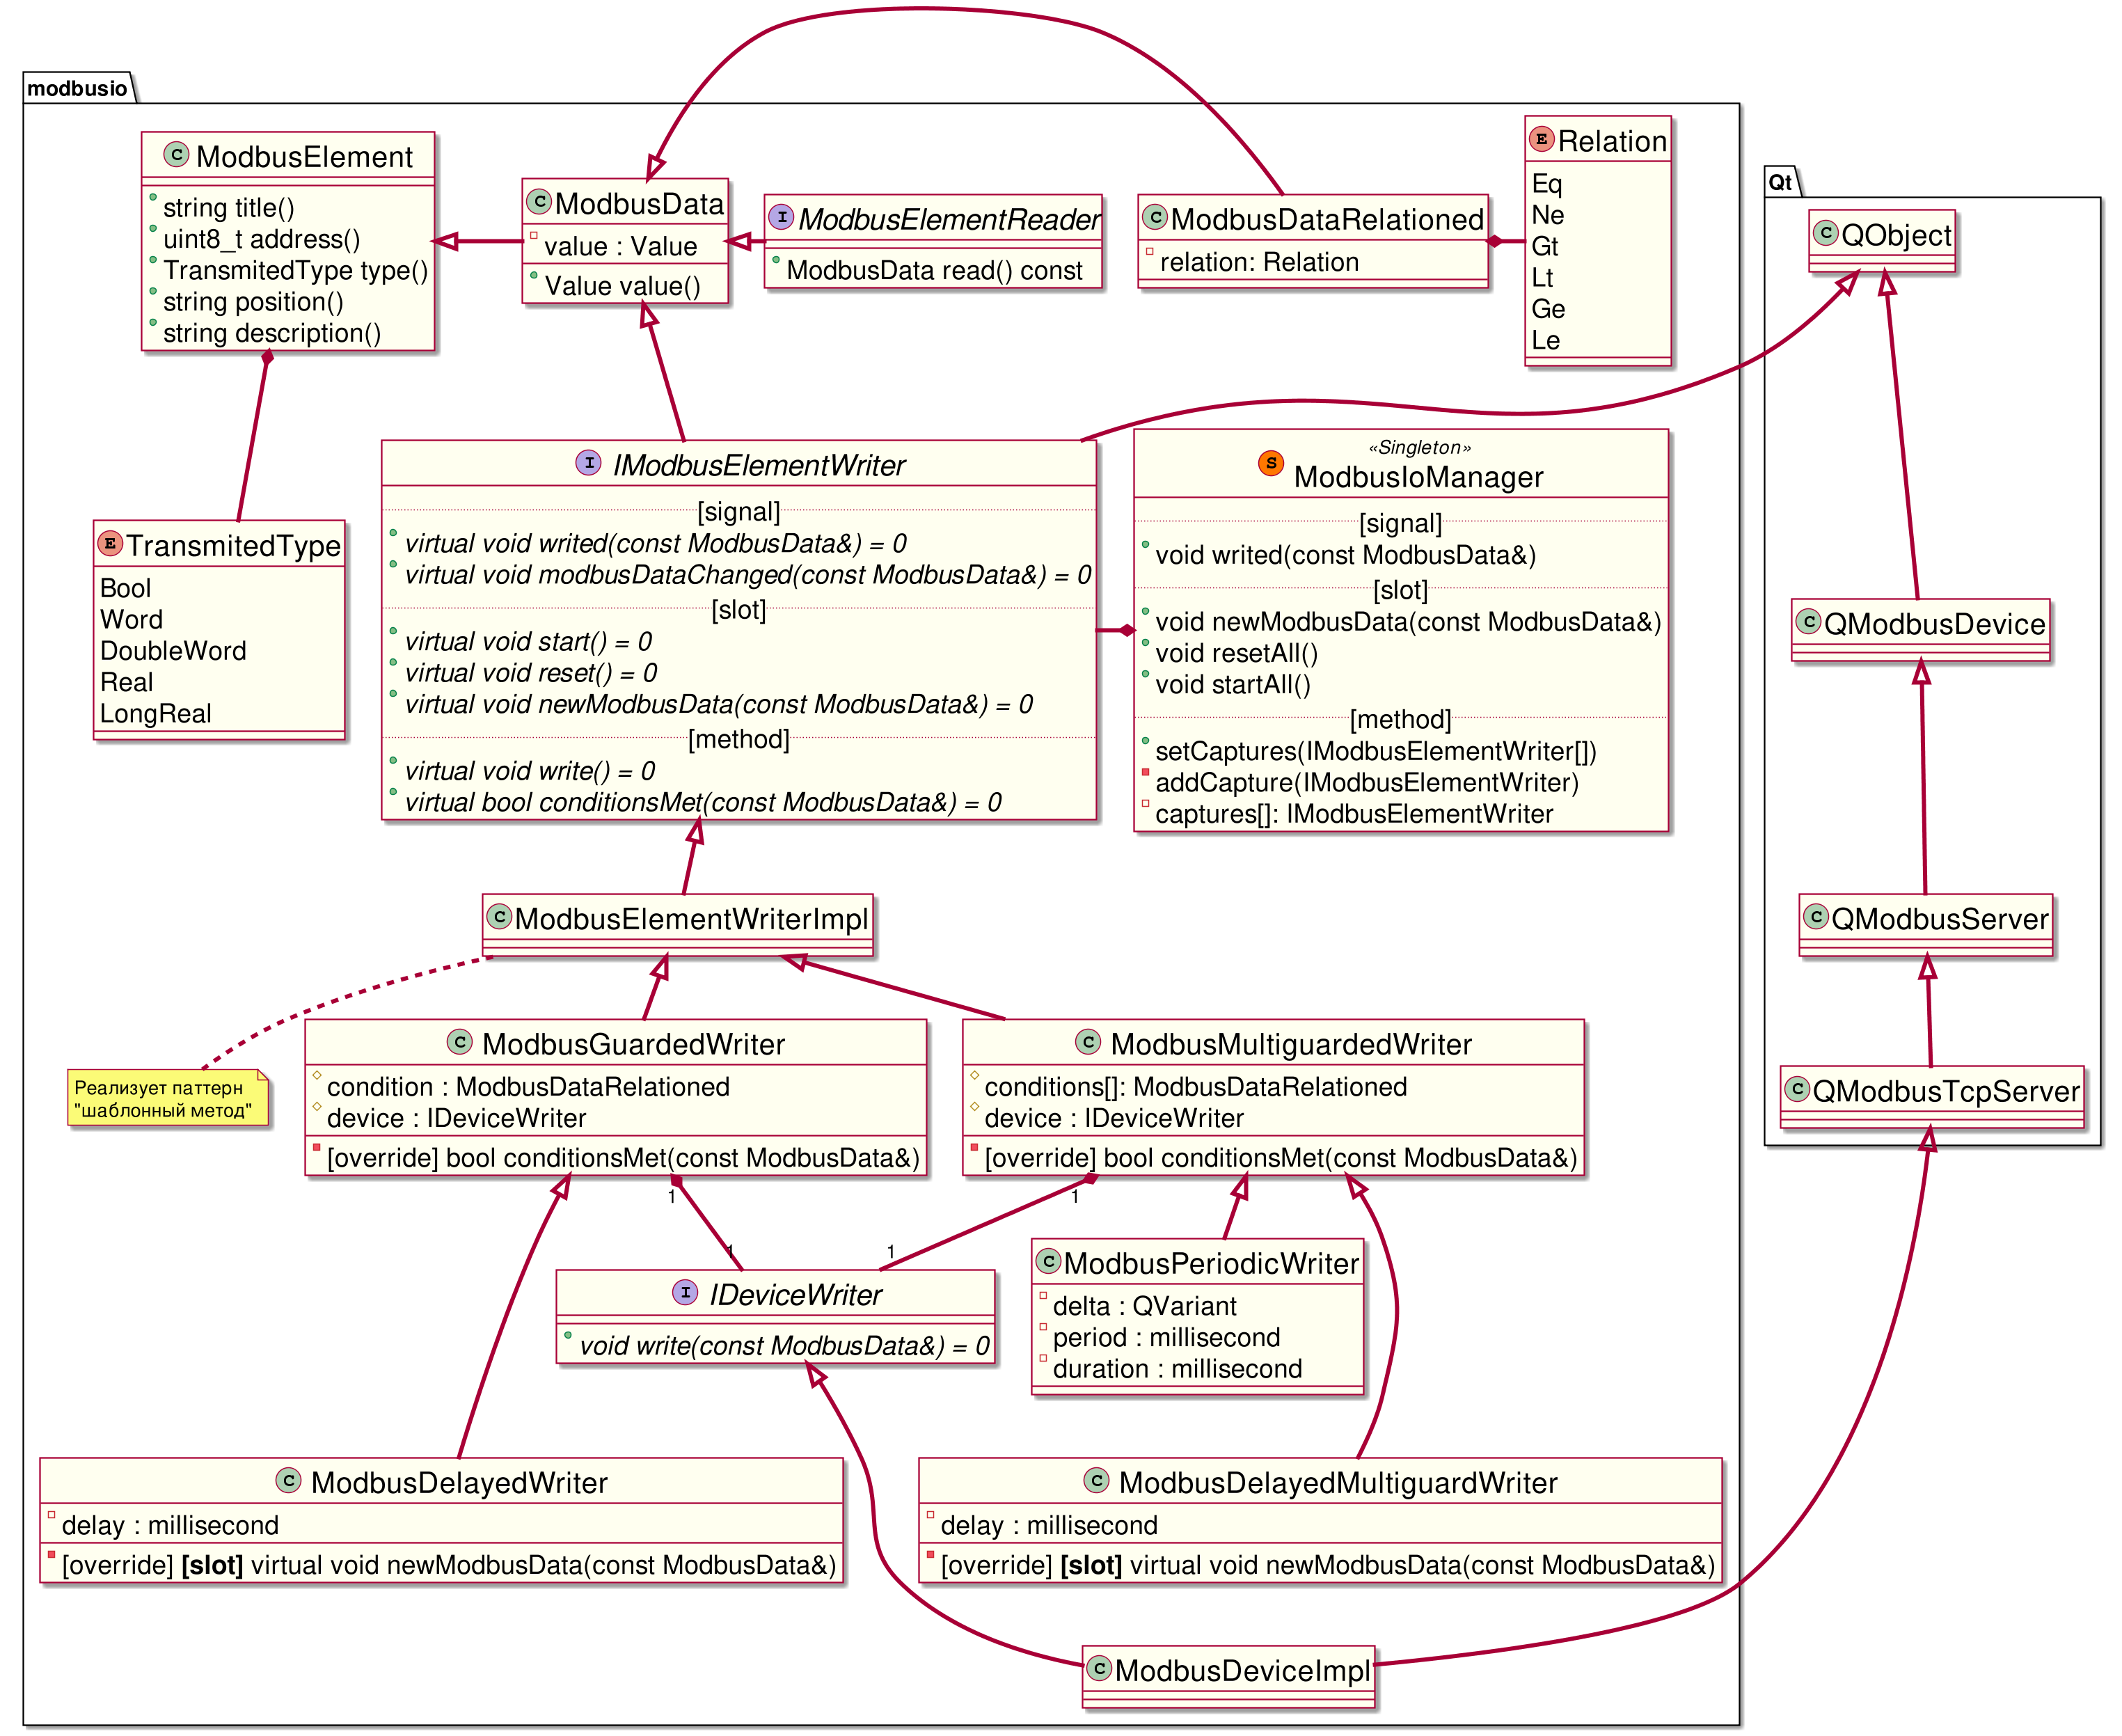
\includegraphics[height=.88\textheight,keepaspectratio]{modbus_class_relationship.png}
    \caption[Иерархия классов имитатора]
        {UML диаграмма классов имитатора модели АНПА при передачи по шине данных типа Modbus.}
            \label{fig:modbus_class_uml}
\end{center}\end{figure}\end{landscape}

Базовый класс \mbelement инкапсулирует в себе представление тега из раздела \ref{sec:modbus_tag}.
Для передачи данных между компонентами системы используется класс \mbdata, производный от \mbelement,
в котором появляется дополнительный член класса \texttt{value} для хранения политипных значений
(то есть для хранения типа \texttt{xsd:aniURI} возможно использовать тип \texttt{std::variant} начиная с \cppseventeen
или его аналог \texttt{QVariant} из библиотеки \texttt{Qt}).
Для реализации поведения используется полиморфизм, так как классы имеют один и тот же протокол \cite[стр. 133]{book:oop:oop_analize}.

Интерфейс \mbreader введен для общности, но в данной работе представляет мало интереса.

\subsection{Жизненный цикл компонента \texttt{IModbusElementWriter}}
Отметим, что этот компонент создается с использованием множественного наследования:
первый супер-класс это \mbdata, инкапсулирующий передаваемые данные,
а второй --- \texttt{QObject}, так как необходимо получить <<ортогональные свойства>>
(механизм сигналов-слотов и обработка сообщений) \cite[стр. 134]{book:oop:oop_analize},
для дальнейшего использования этих возможностей при построении взаимодействий между компонентами.

Каждый экземпляр класса, реализующего интерфейс \mbwriter,
функционирует следующим образом, как показано на рисунке \ref{fig:imodbuselementwriter_activity} \cite[стр. 217]{book:oop:oop_analize}.
После создания, компонент находится в пассивном режиме ожидания, до тех пор пока не будет вызван
метод \texttt{IModbusElementWriter::start()}, после чего компонент подписывается на события шины данных по протоколу Modbus
и слушает сообщения об изменениях значений через слот \texttt{IModbusElementWriter::newModbusData()}.
При поступлении данных, удовлетворяющих условиям функции \texttt{IModbusElementWri\-ter::con\-di\-tions\-Met()},
происходит запись значения через интерфейс \mbdevice (рисунок \ref{fig:modbus_device_imp}),
испускается сигнал \texttt{IModbus\-Ele\-ment\-Writer::writed()},
флаг \texttt{running} выставляется в значение \texttt{false},
а компонент отписывается от событий по шине данных.
Компонент может быть повторно подписан на события, через вызов метода \texttt{IModbusElementWriter::start()}.


\begin{figure}\begin{center}
    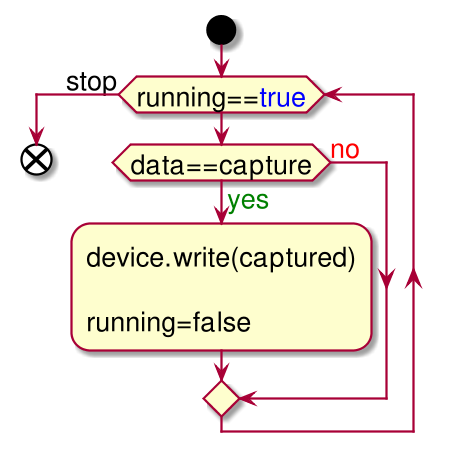
\includegraphics[width=.5\textwidth,keepaspectratio]{imodbuselementwriter_activity}
    \caption[Жизненный цикл компонента \mbwriter]%
        {Жизненный цикл компонента \mbwriter (см. также листинг \ref{lst:tmpl_method_writerimpl}).}%
            \label{fig:imodbuselementwriter_activity}
\end{center}\end{figure}



Класс \texttt{ModbusElementWriterImpl} реализует паттерн <<Шаблонный метод>>\footnote{Template method} \cite[стр. 309]{book:pattern:band_of_4},
определяя метод слота \texttt{IModbusElement\-Writer::new\-Modbus\-Data()}
и защищенный метод \texttt{IModbus\-Element\-Writer::wri\-te()} --- инвариантные последовательности операций,
определенные виртуальными методами, которые уточняются с помощью наследования \cite[стр. 170]{book:tdd:KentBeck}.

\lstinputlisting[
    language=C++,
    caption=Реализация контракта компонента (см. рисунок \ref{fig:imodbuselementwriter_activity}),
    label=lst:tmpl_method_writerimpl
        ]{Dissertation/listings/cpp/writerimpl_template_method.hpp}


\subsection{Условия изменения состояния}
Как видно из рисунка \ref{fig:modbus_class_uml} проверка условий записи описываются с помощью компонента типа
\mbrelationed --- наследника класса \mbdata.
Этот класс содержит в себе \texttt{value} от родительского класса и правило отношения \texttt{Relation},
отражающих свойство \texttt{relation} из таблицы \ref{tbl:modbus_data_properties}.
При поступлении новых данных по шине Modbus происходит сравнение значений (листинг \ref{lst:comparator:compare}),
согласно выражению \eqref{eq:axiom_modbusdatarelationed}.
\lstinputlisting[
    language=C++,
    caption=Вспомогательный метод для анализа поступающих данных,
    label=lst:comparator:compare
        ]{Dissertation/listings/cpp/comparator.hpp}


Перейдем к более подробному рассмотрению реализаций интерфейса \texttt{IModbusElementWriter} его наследниками,
согласно таблице~\ref{tbl:modbuselement_writer_def}.

\subsubsection{Запись с единичным условием}\label{sec:guard}
Циклограмма функционирования класса \texttt{ModbusGuardedWriter} приведена на рисунке \ref{fig:modbus_guarded_writed}.
Этот класс переопределяет метод родительского класса \texttt{IModbusElementWriter::conditionsMet()}.
\begin{figure}[h!]\begin{center}
    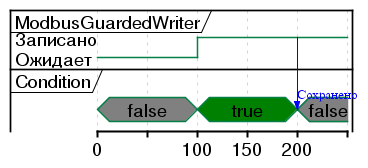
\includegraphics[width=.8\textwidth,keepaspectratio]{modbus_guarded_writer.png}
    \caption[Циклограмма записи значения для единичного условия]
        {Циклограмма записи значения при выполнении условия в момент времени $\tau_1=100$.}
            \label{fig:modbus_guarded_writed}
\end{center}\end{figure}

Как видно из рисунка выполнение условия происходит в момент времени $\tau_1=100$ условных единиц времени,
сразу же по переднему фронту происходит запись нового значения, которое сохраняется даже после окончания
выполнения логического условия \texttt{cond} в $\tau_2=200$.


\subsubsection{Запись со множественными условиями}
Циклограмма функционирования класса \texttt{ModbusMultiguardedWriter} приведена на рисунке \ref{fig:modbus_multiguarded_writed}.
Этот класс переопределяет метод родительского класса \texttt{ModbusElementWriterImpl::newModbusData()},
так как необходимо следить за множеством тегов через этот слот,
заполняется ассоциативный массив (например, \texttt{std::map<std::string, bool>} у которого ключем является
название тега \texttt{modbusio::ModbusElement::title()}, а значением результат выражения
\begin{lstlisting}[language=C++]
    return std::accumulate(list.cbegin(), list.cend(),
        true,
        std::logical_and<>());
\end{lstlisting}
Как видно из рисунка \ref{fig:modbus_multiguarded_writed}, значение не будет записано до тех пор, пока не будут
выполнены все условия, даже если после установления одного из условий оно меняется
(как показано для второго условия на 100 единице времени). Аналогично с \texttt{ModbusGuardedWriter}
после того как значение было записано, выполнение условий не контролируется, 
при этом записанное значение сохраняется, но может быть независимо изменено по другим причинам,
так как компонент больше не владеет ресурсом и отписывается от событий.
\begin{figure}[h!]\begin{center}
    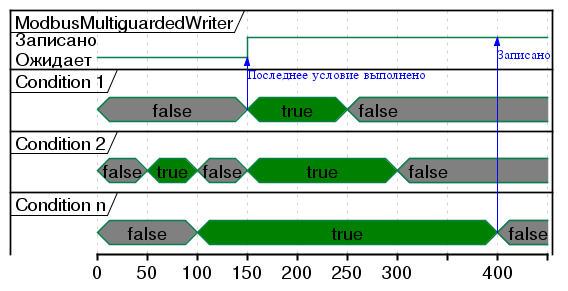
\includegraphics[width=.8\textwidth,keepaspectratio]{modbus_multiguarded_writer.png}
    \caption{Циклограмма записи значения при выполнении множественных условий.}
        \label{fig:modbus_multiguarded_writed}
\end{center}\end{figure}



\subsubsection{Отложенная запись с единичным условием}
Циклограмма функционирования класса \texttt{ModbusDelayedWriter} приведена на рисунке \ref{fig:modbus_delayed_writer}.
Этот класс уточняет метод родительского класса \texttt{ModbusGuardedWriter::conditionsMet()},
при выполнении условия которого запускается таймер на время задержки \texttt{delay},
по окончании которого происходит запись значения.
% \begin{center}
%     \begin{figure}[h!]
%         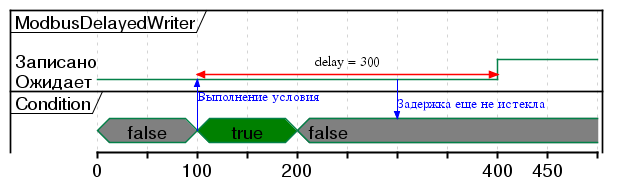
\includegraphics[width=.8\textwidth,keepaspectratio]{modbus_delayed_writer.png}
%         \caption{Циклограмма отложенной записи значения при выполнении единственного условия.}\label{fig:modbus_delayed_writer}
%     \end{figure}
% \end{center}
Класс позволяет устанавливать значение после выполнения условия и по истечению задержки $\tau$.
По окончании таймера на запись значение выражения \texttt{Condition} не анализируется
и запись происходит в любом случае.


\subsubsection{Отложенная запись со множеством условий}
Циклограмма функционирования класса \texttt{ModbusDelayedMultiguardWriter} приведена на рисунке \ref{fig:modbus_delayed_multiguarded_writer}.
Этот компонент переопределяет метод \texttt{IModbusElementWriter::newModbusData()},
а запуск таймера осуществляется при достижении истинного значения
функции супер-класса \texttt{ModbusMultiguardedWriter::conditionsMet()}.

\subsubsection{Периодическая запись}
Данный компонент предназначен для реализации периодических событий, как показано на диаграмме \ref{fig:modbus_periodic_writer}.
При захвате управления дискретной переменной, ее значение инвертируется каждый период
$f_i(x; \tau) = \lnot f_{i-1}(x; \tau)$, причем $f(x; \tau) \in \{0, 1\}$
(на графике сверху захвачен булевский тег, период равен 25 единиц времени, длительность не ограничена).
При захвате вещественной переменной значение меняется по закону
$f_i(x,\Delta x; \tau) = f_{i-1}(x,\Delta x; \tau) + \Delta x, \Delta x \in \mathcal{R}$
(на графике снизу период равен 50 единиц времени, $\Delta x = 10$ на 200 единиц времени).

Этот компонент используется, например, для управления значениями количества оборотов,
количества транзакций и пакетов, переданных от контроллера к программе верхнего уровня,
при захвате вещественных переменной (как уже обсуждалось в разделе \ref{sec:model_anpa_params}).
Очевидно, что приращение $\Delta x$ может быть как положительным, так и отрицательным.

Если в конфигурации сценария (листинг \ref{lst:modbus_periodic_writer_xml}) имеется атрибут
\texttt{duration}, компонент будет работать от выполнения условий до окончания указанной длительности.
В противном случае обновление значений будет происходить до момента прекращения работы
путем вызова функции \texttt{IModbusElementWriter::reset()}.

\begin{figure}[h!]\begin{center}
    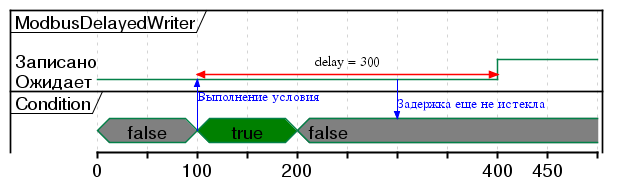
\includegraphics[width=.8\textwidth,keepaspectratio]{modbus_delayed_writer.png}
    \caption{Циклограмма отложенной записи значения при выполнении единственного условия.}\label{fig:modbus_delayed_writer}
    %
    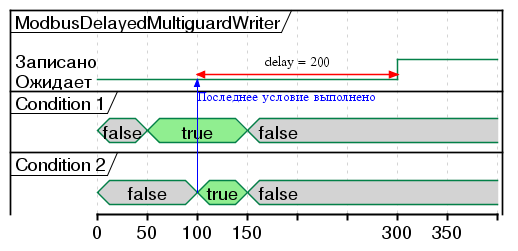
\includegraphics[width=.8\textwidth,keepaspectratio]{modbus_delayed_multiguarded_writer.png}
    \caption{Циклограмма отложенной записи значения при выполнении множественных условий.}\label{fig:modbus_delayed_multiguarded_writer}
    %
    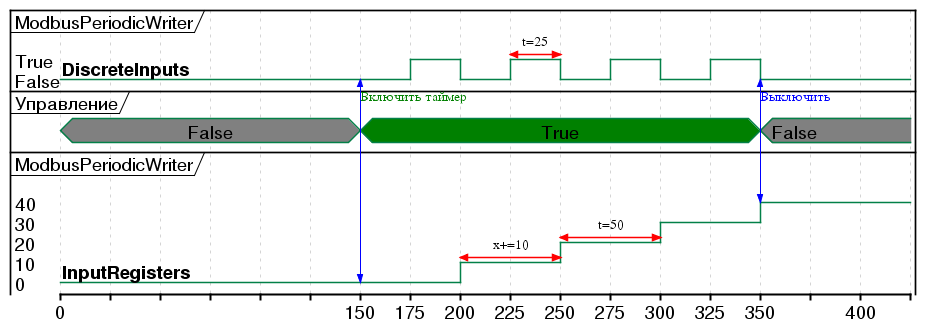
\includegraphics[width=.8\textwidth,keepaspectratio]{modbus_periodic_writer.png}
    \caption{Циклограмма периодической записи значения.}\label{fig:modbus_periodic_writer}
\end{center}\end{figure}



\subsection{Реализация интерфейса \mbdevice}
Для реализации интерфейса \mbdevice также используется возможность множественного наследование языка программирования \cpp:
одним из родителей является интерфейс \mbdevice,
а вторым --- класс библиотеки~\texttt{Qt}, обеспечивающий реализацию физической передачи информации по протоколу Modbus
\texttt{QModbusTcpServer}, так как обмен происходит по разновидности протокола Modbus TCP/IP.
Упрощенная реализация показана в листинге~\ref{lst:imodbus_device_impl}.
\begin{figure}[hb!]\begin{center}
        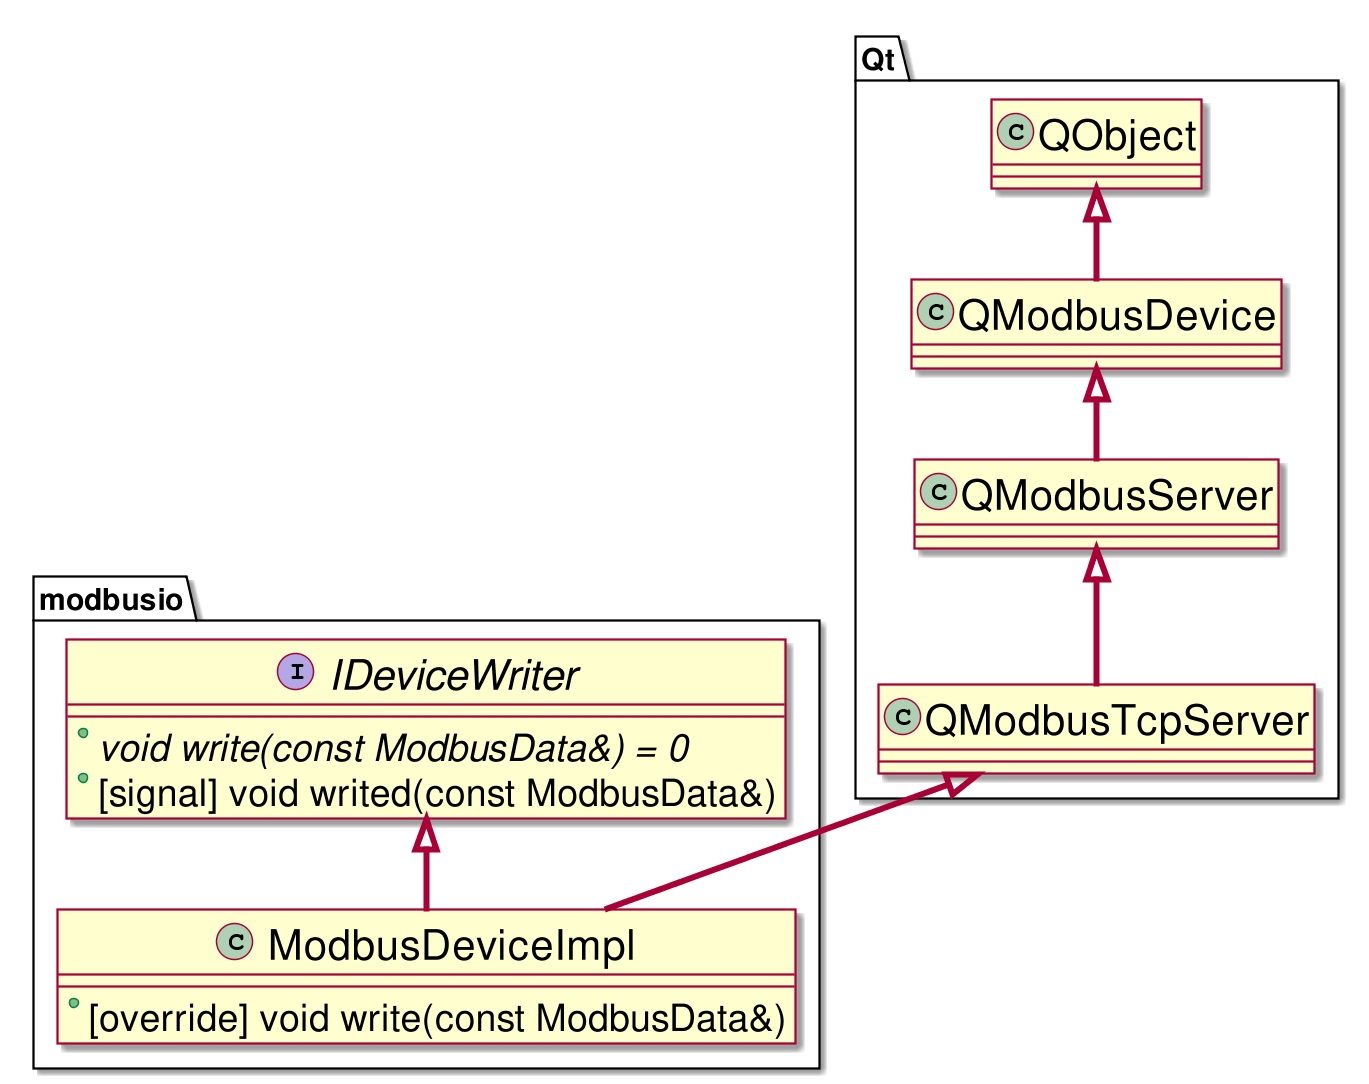
\includegraphics[width=.6\textwidth,keepaspectratio]{modbus_device_impl.png}
        \caption[Реализация интерфейса устройства записи.]
            {Реализация устройства для записи значений по протоколу Modbus.}\label{fig:modbus_device_imp}
\end{center}\end{figure}
\lstinputlisting[
    language=C++,
    caption=Простейшая реализация \mbdevice устройства,
    label=lst:imodbus_device_impl]
        {Dissertation/listings/cpp/dummydeviceimpl.hpp}
Таким образом используется интерфейс вместо конкретной реализации \cite[стр. 47-48]{book:pattern:head_first}


\subsection{Описание конфигурационного файла для компонентов интерфейса \mbwriter}
Каждая группа должна быть помещена в корневой элемент \texttt{Scenario},
как показано в листинге \ref{lst:modbus_scenario_example_diagram} приложения \ref{app:sec:modbus_scenario_example_diagram}.
%
Каждый компонент помещается внутри тега \texttt{Writer} (представляющий класс всех возможных изменений $\mathbb{A}$ из раздела \ref{sec:ontology}),
с обязательным текстовым атрибутом \texttt{tag}, который указывает каким ресурсом владеет данный компонент
и обязательным атрибутом \texttt{value} (см. листинг~\ref{lst:modbus_tags_scenario_configs}).
Также есть ряд необязательных атрибутов, о которых будет сказано отдельно. 
Одновременно владеть одним и тем же ресурсом могут несколько компонентов,
так как у одного и того же компонента может быть множество причин для изменений -- изоморфны.
Далее следует секция условий --- \texttt{Conditions},
описывающая классы отношений $\mathbb{C}$ (см. также выражение~\eqref{eq:axiom_modbusdatarelationed}).
Каждое условие описывается логической операцией отношения \texttt{relation} для смежного параметра,
указанного в обязательном поле \texttt{tag} и связанного с ним обязательном значении \texttt{value}.
Необязательный атрибут \texttt{relation} принимает одно из следующих значений:
\texttt{eq}~($=$),
\texttt{ne}~($\neq$),
\texttt{gt}~($>$),
\texttt{lt}~($<$),
\texttt{ge}~($\geq$),
\texttt{le}~($\leq$), по аналогии с обозначениями в языке Fortran.
Отношение типа \texttt{eq} считается отношением по умолчанию,
все остальные отношения же необходимо указывать явным образом.
Необязательным полем является атрибут \texttt{Purpose}, в котором размещается информация для
обозначения назначения компонента в сценарии. 


\subsubsection{ModbusGuardedWriter}
Рассмотрим более подробно описание компонента для записи с единичным условием,
который размещается в элементе \texttt{Guarded} листинга~\ref{lst:modbus_guarded_writer_xml}:
\lstinputlisting[
    language=MyXML,
    caption=Пример конфигурации \texttt{ModbusGuardedWriter},
    label=lst:modbus_guarded_writer_xml]
        {Dissertation/listings/xml/guarded.xml}
Захватывается управление над тегом \texttt{A1}, которой будет присвоено значение 160
при выполнении условия \texttt{R1 = true}.
Иными словами при истинности предиката $P$ будет выполнено действие $Q$:
$P(R1=\mbox{true}) \to Q(A1=160)$.


\subsubsection{ModbusMultiguardedWriter}
Для описания компонента со множественными условиями, используется следующий формат,
который размещается в элементе \texttt{Multiguarded} листинга~\ref{lst:modbus_multiguarded_writer_xml}:
\lstinputlisting[
    language=MyXML,
    caption=Пример конфигурации \texttt{ModbusMultiguardedWriter},
    label=lst:modbus_multiguarded_writer_xml]
        {Dissertation/listings/xml/multiguarded.xml}
Переменной \texttt{Regime} будет присвоено значение 1, как только 
одновременно будет выполнено два условия: $Regime = 1: \{A1 \ge 150 \wedge C1 = true\}$.
Таким образом $P(x_1,\ldots,x_n) = P(A1\ge150, C1=\mbox{true}) \to Q(Regime=1)$.

\subsubsection{ModbusDelayedWriter и ModbusDelayedMultiguardWriter}
Компоненты этого типа располагаются в окружении тегов элементов \texttt{DelayedGuarded} и \texttt{DelayedMultiGuarded}, соответственно,
как показано в листинге~\ref{lst:modbus_delayed_writer_xml}.
\lstinputlisting[
    language=MyXML,
    caption=Пример конфигурации \texttt{ModbusDelayedWriter} и \texttt{ModbusDelayedMultiguardWriter},
    label=lst:modbus_delayed_writer_xml]
        {Dissertation/listings/xml/delayed.xml}
Очевидно, что происходит захват управления значения переменной \texttt{PP\_1}, которой будет установлено значение \texttt{true}
через 50 единиц времени, как только будут выполнены два условия:
$PP\_1 = \mbox{true}: \{R1 = \mbox{true} \wedge A1 \le 150\}$.
Или используя предикатные обозначения
$P(x_1,\ldots,x_n) = P(A1\le150, R1=\mbox{true}, \tau=50) \to Q(PP\_1=\mbox{true})$.


\subsubsection{ModbusPeriodicWriter}
Данный компонент располагается внутри элемента \texttt{Period} в конфигурационном файле сценария,
согласно листингу~\ref{lst:modbus_periodic_writer_xml}.
\lstinputlisting[
    language=MyXML,
    caption=Пример конфигурации \texttt{ModbusPeriodicWriter},
    label=lst:modbus_periodic_writer_xml]
        {Dissertation/listings/xml/periodic.xml}
В данном примере дистанция, ассоциированная с переменной \texttt{Distance}, увеличивается на 100 единиц каждые 1000 единиц времени,
при выполнении ряда условий, а именно: $\{C1 = true \wedge A1 > 100 \wedge A1 \le 150 \}$ или
увеличивается на теже 100 единиц, но с периодом 500 единиц, когда достигаются следующие условия:
$\{C1 = true \wedge A1 > 150\}$
Отметим, что для этого компонента начальное значение устанавливается с помощью атрибута \texttt{value}
при вызове метода \texttt{IModbusElementWriter::start()}.


\subsection{Сводная таблица наследников \texttt{IModbusElementWriter}}
Общая информация о компонентах представлена в таблице~\ref{tbl:ModbusElementWriterImpl}.
Из этой таблицы видно, что использование наследования совместно с паттерном <<шаблонный метод>>
позволяет переопределять поведение компонентов, обеспечивая выполнение контрактов наследниками интерфейса
\cite[стр. 124-125]{book:oop:oop_analize,bib:my:ttd_with_patterns_2019}.

\begin{table}[h!]
\begin{center}
\caption{Сводная таблица \textit{метаклассов} модели АНПА.}\label{tbl:ModbusElementWriterImpl}
\begin{tabular}{|l|c|c|c|c|c|c||c|c|}
\hline
    \multicolumn{1}{|c|}{\multirow{2}{*}{Наследники}} &
    \multicolumn{6}{c||}{\textbf{атрибуты}} &
    \multicolumn{2}{c|}{\textbf{override}} \\ \cline{2-9} %Переопределенные методы наследника
    \multicolumn{1}{|c|}{}     &
        \rotatebox{90}{tag} & \rotatebox{90}{value}  & \rotatebox{90}{delay}  & \rotatebox{90}{period} &
        \rotatebox{90}{delta} & \rotatebox{90}{duration} &
        \rotatebox{90}{conditionsMet} & \rotatebox{90}{newModbusData} \\ \hline
    \texttt{ModbusGuardedWriter}              & +    & +      & -      & -      & - &-     & + & -  \\ \hline
    \texttt{ModbusMultiguardedWriter}         & +    & +      & -      & -      & - &-     & + & -  \\ \hline
    \texttt{ModbusDelayedWriter}              & +    & +      & +      & -      & - &-     & - & +  \\ \hline
    \texttt{ModbusDelayedMultiguardWriter}    & +    & +      & +      & -      & - &-     & - & +  \\ \hline
    \texttt{ModbusPeriodicWriter}             & +    & +      & -      & +      & + &$\pm$ & + & -  \\ \hline
\end{tabular}
\end{center}
\end{table}


\section{Менеджер индивидов класса \mbwriter имитатора}
Для управления компонентами имитатора используется менеджер компонентов \texttt{ModbusIoManager}.
Установка компонентов производится с помощью экземпляра класса \texttt{ScenarioParser}, реализующего интерфейс \texttt{IParser}.
Этот интерфейс является общим как для чтения файла сценария (листинг~\ref{lst:modbus_scenario_example_diagram}),
так и для файла тегов (листинг \ref{lst:modbus_tags_example}).
При чтении конфигурации проверяется, что каждый тег $t_i$ типа \mbdata,
управление над которым захватывается, или условия выполнения переходов типа \mbrelationed,
являются элементами множества класса первичных данных, то есть $\forall t_i \in \mathbb{T}$ (см. раздел \ref{sec:ontology}).

На рисунке \ref{fig:modbus_class_components} показано отношение между менеджером \texttt{ModbusIoManager},
интерфейсом парсера \texttt{IParser} и интерфейсом \mbwriter.
\begin{center}
    \begin{figure}[hb!]
        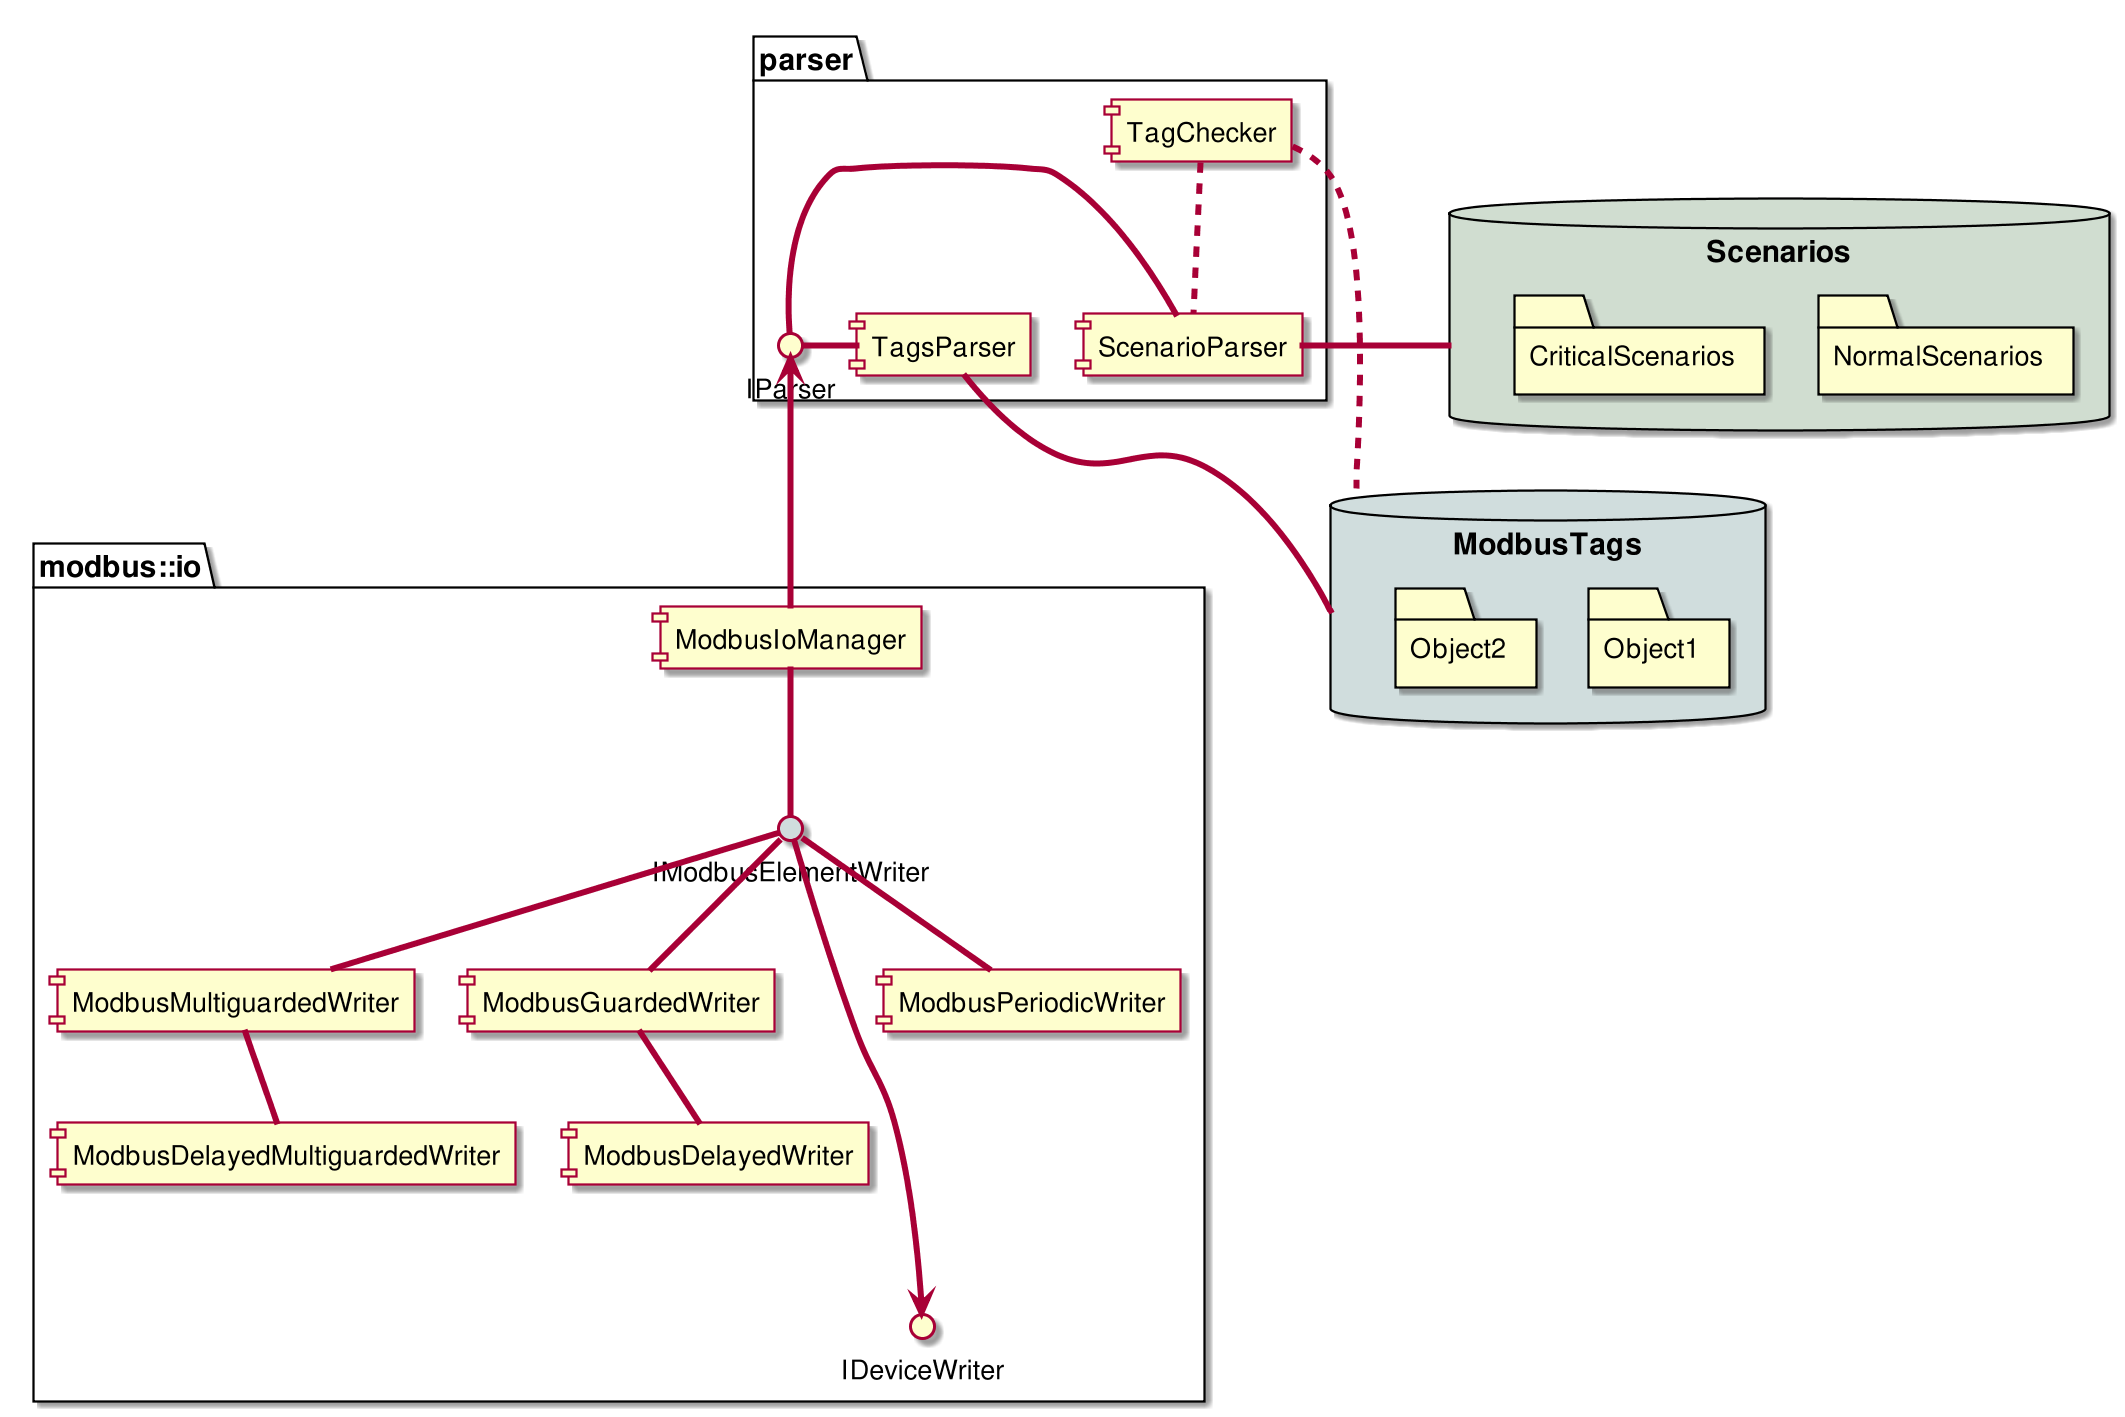
\includegraphics[width=.9\textwidth,keepaspectratio]{modbus_class_components}
        \caption{Композиция классов менеджера сценариев.}\label{fig:modbus_class_components}
    \end{figure}
\end{center}


Последовательность действий по конфигурированию окружения программного обеспечения
показана на рисунке~\ref{fig:top_level_sequence} \cite[стр. 239]{book:oop:oop_analize}.
\begin{center}
    \begin{figure}
        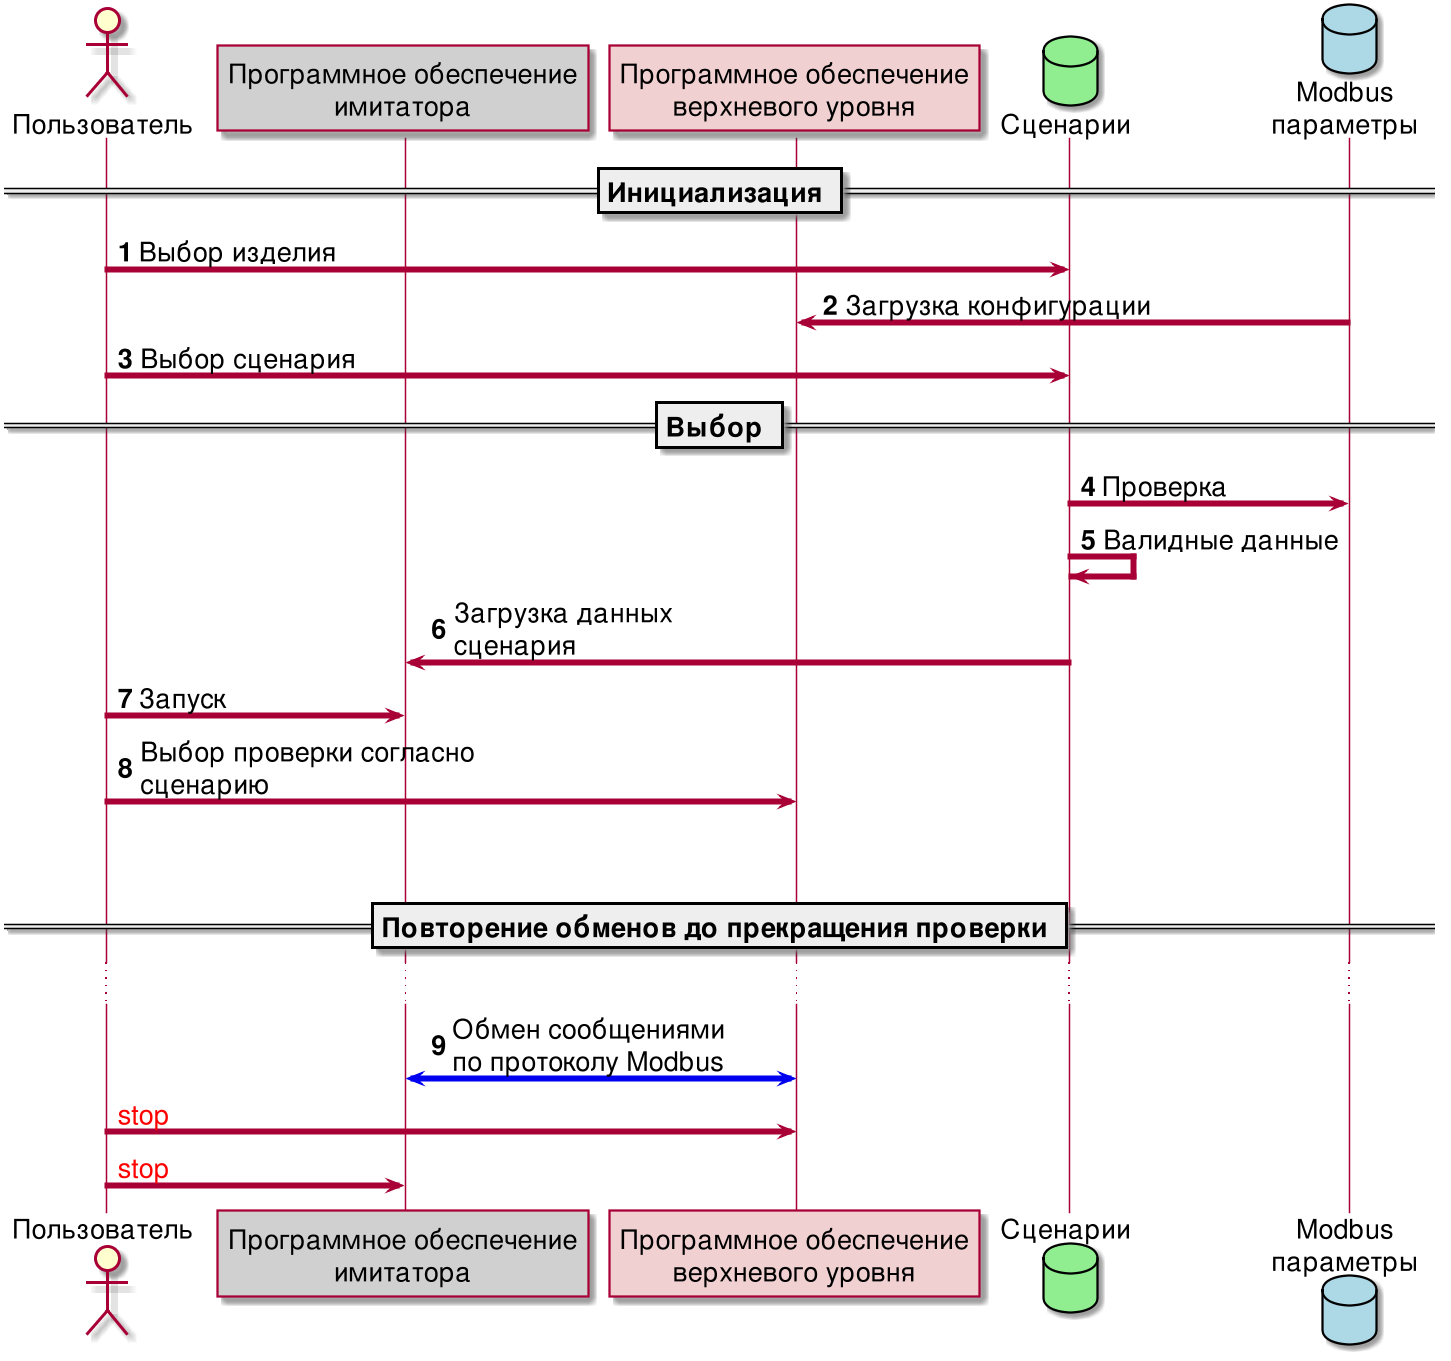
\includegraphics[width=.9\textwidth,keepaspectratio]{top_level.png}
        \caption{Последовательность действий при работе с имитатором}
        \label{fig:top_level_sequence}
    \end{figure}
\end{center}

\textbf{Инициализация и загрузка конфигурации.}
На этом этапе происходит настройка программного обеспечения
имитатора и программы, так называемого, верхнего уровня,
то есть программного обеспечения непосредственно системы контроля.
В случае корректной конфигурации происходит запуск
выбранной проверки оператором.

\textbf{Выполнение сценария проверки.}
После запуска две программы начинают обмениваться 
сообщениями по протоколу Modbus~TCP/IP, например внутри локальной сети.
Более подробно этот этап показан на рисунке \ref{fig:modbuselementwriterimpl}.

\textbf{Окончание проверки.}
Происходит возврат к исходным настройкам систем и отключение.
После этого процедура может быть воспроизведена вновь с теми же
или другими параметрами. 

\begin{center}
    \begin{figure}
        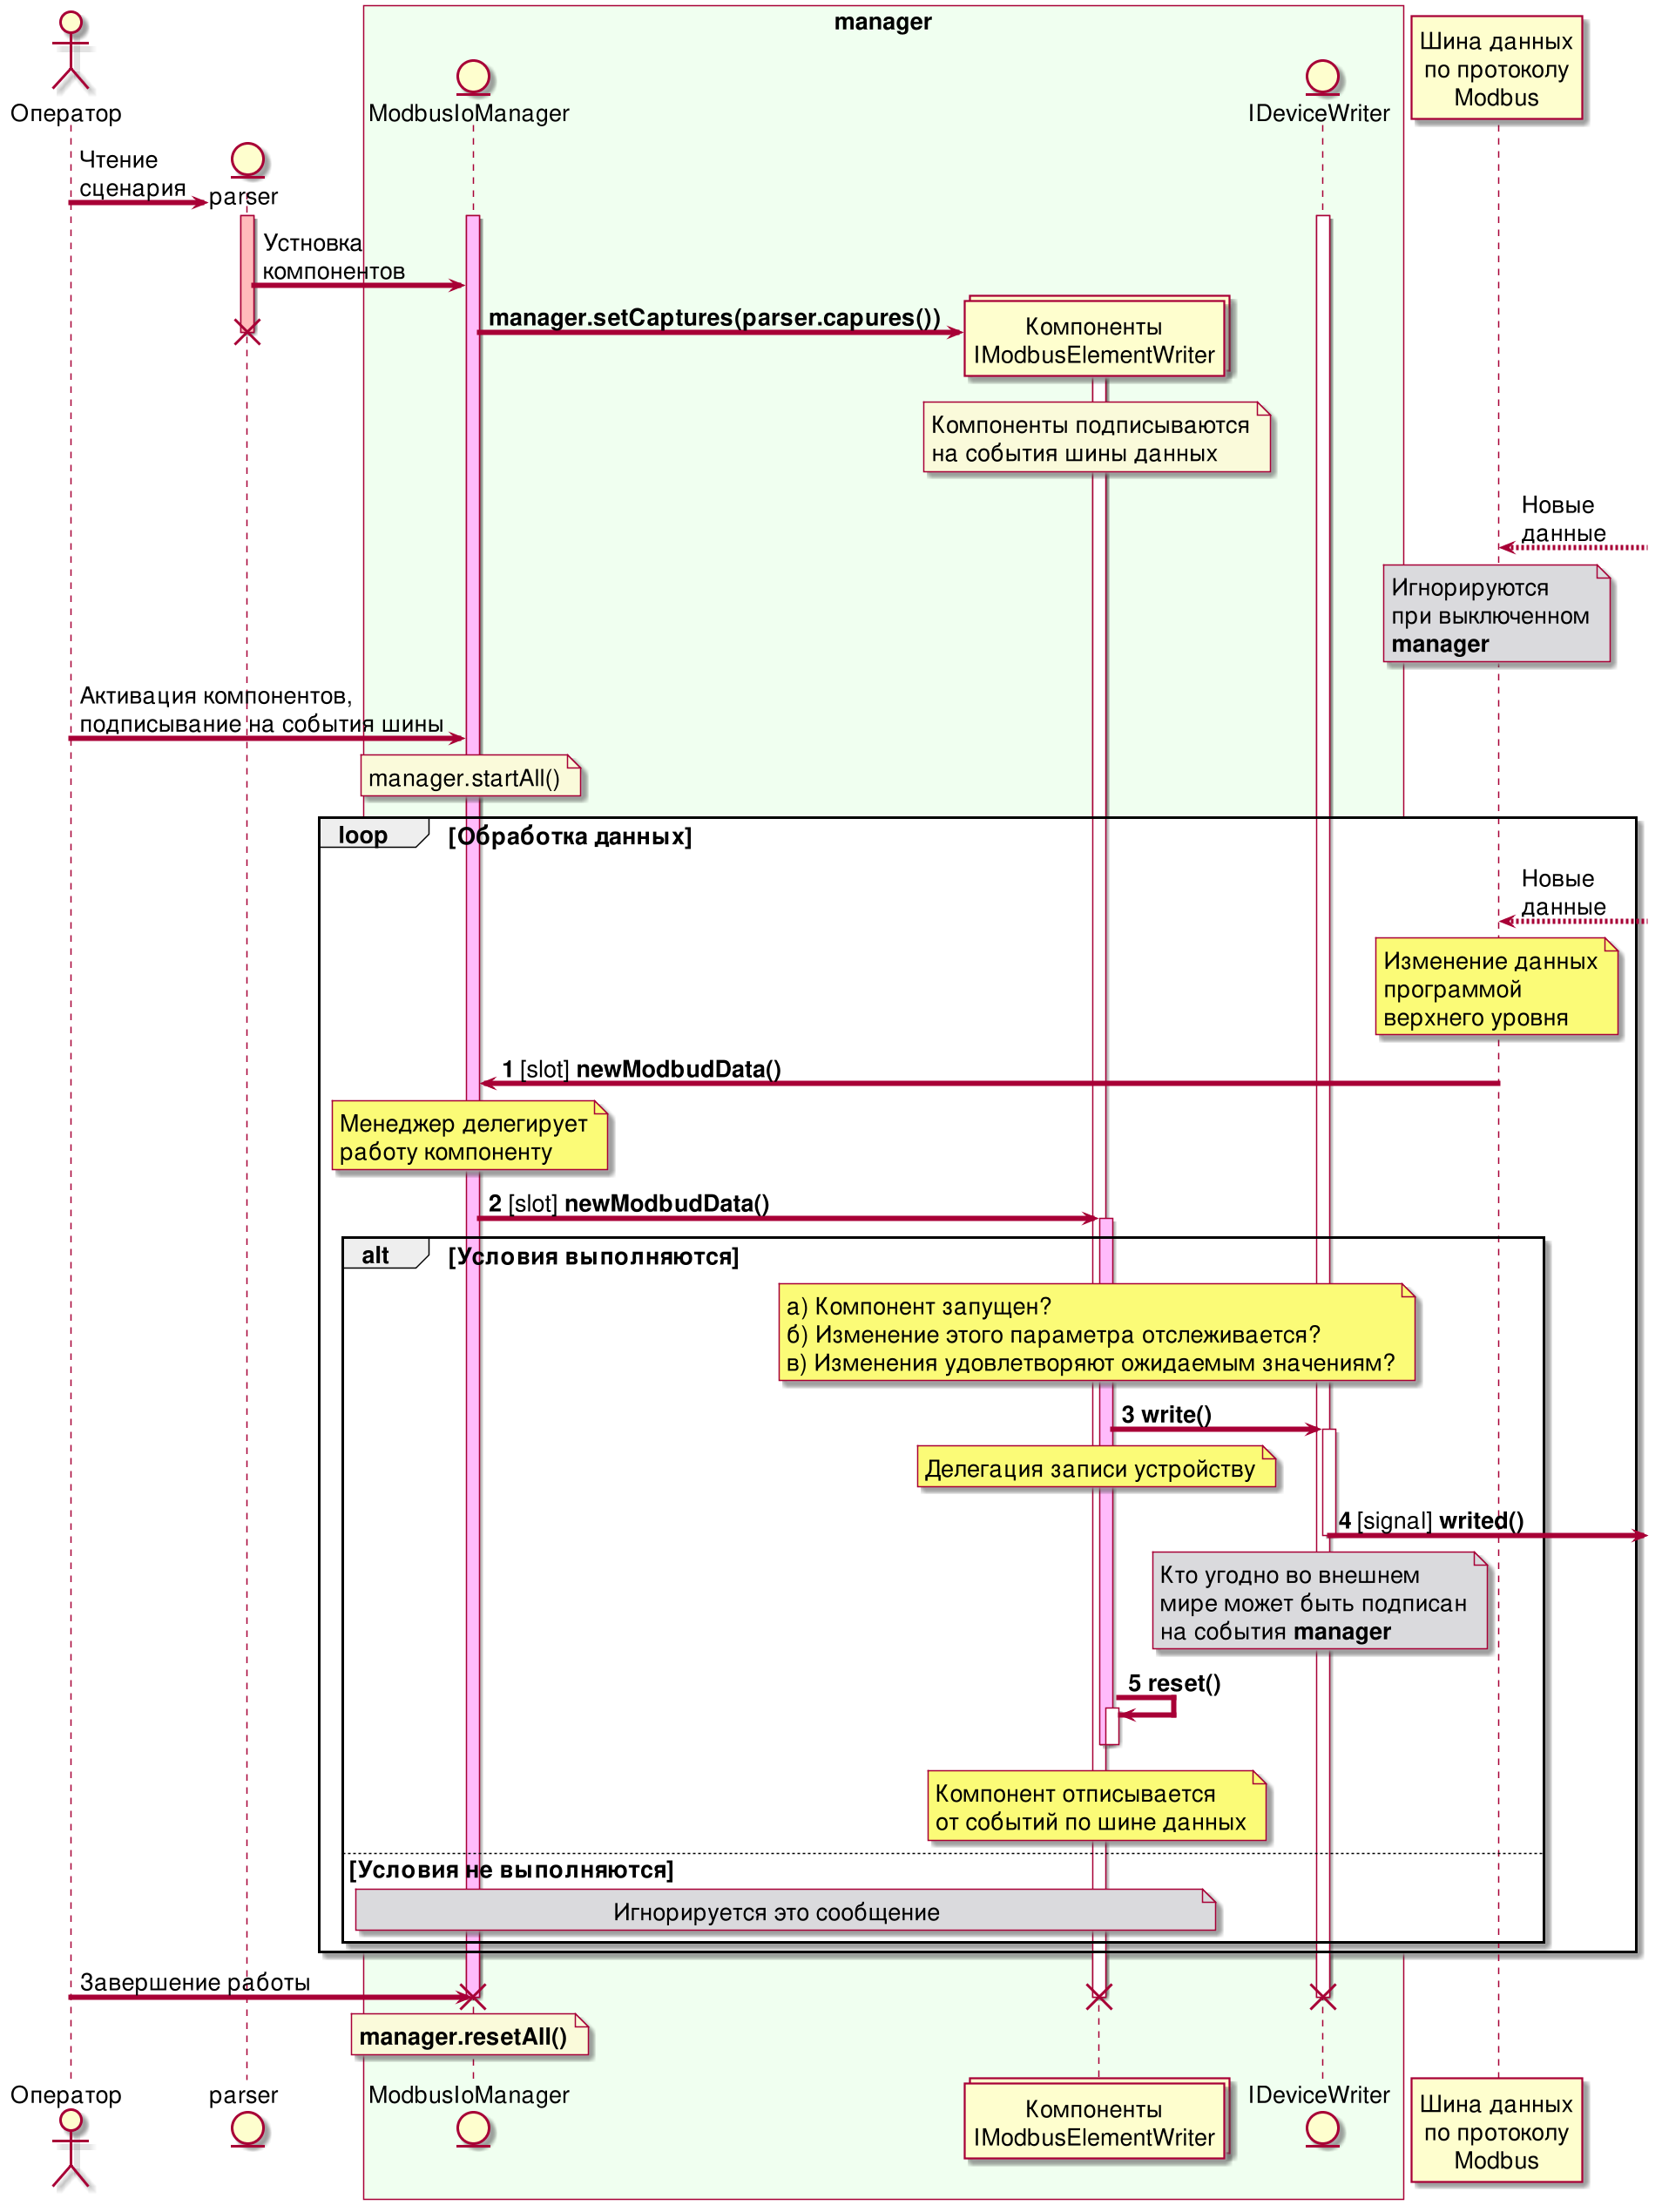
\includegraphics[height=.8\textheight,keepaspectratio]{modbuselementwriterimpl.png}
        \caption[Взаимодействие компонентов с шиной данных]
            {Взаимодействие компонентов с шиной данных (см. также листинг \ref{lst:tmpl_method_writerimpl})}
        \label{fig:modbuselementwriterimpl}
    \end{figure}
\end{center}


\textbf{Обработка данных при выполнении сценария проверки.}
Как было сказано ранее, после запуска менеджера \texttt{modbusio::\-ModbusIoManager::\-start\-All()}
менеджер готов к обработке данных.
До этого момента приходящие сообщения игнорируются им.

Таким образом, менеджер подписывается на изменения данных по шине Modbus,
через слот \texttt{newModbusData()}.
Работа с поступающими данными делегируется экземплярам, реализующих интерфейс
\mbwriter, после чего происходит проверка поступающих данных по следующим пунктам.
\begin{enumerate}
    \item Запущен ли компонент.
    \item Изменение это параметра отслеживается. Как было сказано ранее в разделе \ref{sec:ontology}
        два и более компонентов могут быть изоморфны относительно входного сигнала,
        таким образом, очевидно что этот сигнал перенаправляется всем компонентам,
        которыми владеет менеджер.
    \item Происходит проверка все ли предикаты в правилах перехода в значении истина. 
\end{enumerate}
При выполнении всех трех пунктов хотя бы для одного компонента,
происходит запись значения $P(x_1, \ldots, x_n) \to Q(x)$.
Компонент делегирует это экземпляру, реализующему интерфейс \mbdevice,
через вызов виртуальной функции \texttt{IDeviceWriter::write()}.
В следствии этого компонент отписывается от событий по шине данных,
вызовом функции \texttt{IModbusElementWriter::reset()}.

Обработка данных при выполнении сценария проверки происходит до тех пор
пока менеджер не будет остановлен \texttt{ModbusIoManager::resetAll()}.


\section{Пример композиции для простейшего сценария}

Рассмотрим пример сценария на основе множества Modbus тегов из листинга \ref{lst:modbus_tags_example},
циклограмма которого представлена на рисунке \ref{fig:modbus_scenario_example_diagram},
сценарий приведен в листинге \ref{lst:modbus_scenario_example_diagram} в разделе приложения \ref{app:sec:modbus_scenario_example_diagram}.
Схема разметки приведена в листинге \ref{lst:modbus_tags_scenario_configs}.

\begin{landscape}
    \begin{center}
        \begin{figure}
            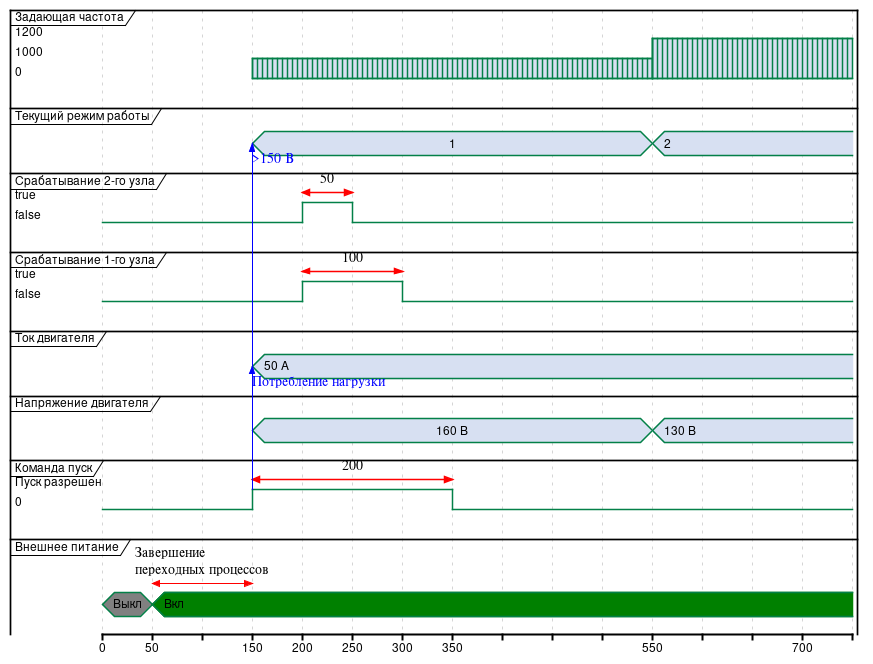
\includegraphics[height=.8\textheight,keepaspectratio]{modbus_scenario_example_diagram.png}
            \caption{Пример использования классов.}\label{fig:modbus_scenario_example_diagram}
        \end{figure}
    \end{center}
\end{landscape}


\clearpage\section*{Заключение по главе \thechapter}
Продемонстрирован унифицированный способ представления субъектно-ориентированного механизма
изменения параметров, для имитации как внешнего так и внутреннего окружения объекта контроля.
Создана онтологическая модель автономного необитаемого подводного аппарата.
На основе проведенных исследований модели создана программная реализация 
с использованием языка программирования \cpp и библиотки \texttt{Qt}.

Разработанное специализированное программное обеспечение имитатора 
в своей работе использует те же сущности предметной области (теги из листинга~\ref{lst:modbus_tags_example}),
что и программное обеспечение автоматизированных систем контроля и диагностики.           % Глава 3
\chapter*{Заключение}                       % Заголовок
\addcontentsline{toc}{chapter}{Заключение}  % Добавляем его в оглавление

%% Согласно ГОСТ Р 7.0.11-2011:
%% 5.3.3 В заключении диссертации излагают итоги выполненного исследования, рекомендации, перспективы дальнейшей разработки темы.
%% 9.2.3 В заключении автореферата диссертации излагают итоги данного исследования, рекомендации и перспективы дальнейшей разработки темы.
%% Поэтому имеет смысл сделать эту часть общей и загрузить из одного файла в автореферат и в диссертацию:

Основные результаты работы заключаются в следующем.
%% Согласно ГОСТ Р 7.0.11-2011:
%% 5.3.3 В заключении диссертации излагают итоги выполненного исследования, рекомендации, перспективы дальнейшей разработки темы.
%% 9.2.3 В заключении автореферата диссертации излагают итоги данного исследования, рекомендации и перспективы дальнейшей разработки темы.
\begin{enumerate}
  \item Был произведен графоаналитический анализ модели автономного необитаемого подводного аппарата для выявления
      общесистемных объектов.
  %
  \item Была произведена декомпозиция модели автономного необитаемого подводного аппарата на основе результатов
      графоаналитического анализа с целью выделения метаклассов.
  %
  % \item Численные исследования показали, что \ldots
  % \item Математическое моделирование показало \ldots
  \item Для выполнения поставленных задач был создан программный комплекс имитатора абонентов сети Modbus.
  %
  \item На предприятии \leadingOrganizationTitle была произведена апробация результатов разработки программного комплекса,
      что подтверждается соответствующим актом о внедрении.
  %
  \item Было получено свидетельство о государственной регистрации программы для ЭВМ.
\end{enumerate}

И какая-нибудь заключающая фраза.

Последний параграф может включать благодарности.  В заключение автор
выражает благодарность и большую признательность научному руководителю
Коромысличенко~В.\:Н. за поддержку, помощь, обсуждение результатов и~научное
руководство. Также автор благодарит Бойдало~М.\:К. за помощь в~редактировании текста.
Автор также благодарит много разных людей и~всех, кто сделал настоящую работу автора возможной.
      % Заключение
\chapter*{Список сокращений и условных обозначений} % Заголовок
\addcontentsline{toc}{chapter}{Список сокращений и условных обозначений}  % Добавляем его в оглавление
\noindent
% \begin{longtabu} to \dimexpr \textwidth-5\tabcolsep {r X}
\begin{longtabu} to \textwidth {r X}
    $\mathcal{M}$ & Множество дискретных и аналоговых параметров, передаваемых по сети Modbus \\
    %
    %
    \textbf{АНПА} & Автономный необитаемый подводный аппарат \\
    \textbf{АСУ~ТП} & Автоматизированная система управления технологическим процессом \\
    \textbf{БГР} & Блок гальванической развязки \\
    \textbf{ВУ} & Верхний уровень \\
    \textbf{НУ} & Нижний уровень \\
    \textbf{ОК} & Объект контроля \\
    \textbf{ПЛК} & Программируемый логический контроллер \\
    \textbf{ПО} & Программное обеспечение \\
    \textbf{СИ} & Синхроимпульс \\
    \textbf{СК} & Система контроля \\
    \textbf{ЭВМ} & Электронно-вычислительная машина \\
    \textbf{RDF} & Resource description framework \\
\end{longtabu}
\addtocounter{table}{-1}% Нужно откатить на единицу счетчик номеров таблиц, так как предыдующая таблица сделана для удобства представления информации по ГОСТ
        % Список сокращений и условных обозначений
\chapter*{Словарь терминов}             % Заголовок
\addcontentsline{toc}{chapter}{Словарь терминов}  % Добавляем его в оглавление

% \textbf{TeX} : Cистема компьютерной вёрстки, разработанная американским профессором информатики Дональдом Кнутом

% \textbf{панграмма} : Короткий текст, использующий все или почти все буквы алфавита
      % Словарь терминов
\include{Dissertation/references}      % Список литературы
\include{Dissertation/lists}           % Списки таблиц и изображений (иллюстративный материал)

%%% Настройки для приложений
\appendix
% Оформление заголовков приложений ближе к ГОСТ:
\setlength{\midchapskip}{20pt}
\renewcommand*{\afterchapternum}{\par\nobreak\vskip \midchapskip}
\renewcommand\thechapter{\Asbuk{chapter}} % Чтобы приложения русскими буквами нумеровались

\begin{landscape}
\chapter{Листинги}
\section{Конфигурационный файл параметров сети Modbus}\label{app:sec:modbus_tag}
    \lstinputlisting[
        language=MyXML,
        caption=Конфигурационный файл для описания множества контроллируемых параетров по промышленному протоколу Modbus
            из раздела \ref{sec:modbus_tag}. Файл разметки приведен в листинге \ref{lst:modbus_tags_example_configs},
        label=lst:modbus_tags_example]
            {Dissertation/listings/xml/modbus_tags_example.xml}
\end{landscape}

\section{Конфигурация сценария}\label{app:sec:modbus_scenario_example_diagram}
\lstinputlisting[
    language=MyXML,
    caption=Конфигурационный файл примера сценария развития событий (см. рисунок \ref{fig:modbus_scenario_example_diagram}),
    label=lst:modbus_scenario_example_diagram]
        {Dissertation/listings/xml/modbus_tags_example_scenario.xml}

\begin{landscape}
\section{\todo{XSD} файлы}\label{app:sec:xsd}
    \lstinputlisting[
        language=MyXML,
        caption=\todo{modbus scheme},
        label=lst:modbus_tags_example_configs]
            {Dissertation/listings/xsd/modbus_tags_configs.xsd}
    
    \lstinputlisting[
        language=MyXML,
        caption=\todo{modbus scenario scheme},
        label=lst:modbus_tags_scenario_configs]
            {Dissertation/listings/xsd/modbus_tags_scenario_configs.xsd}        
\end{landscape}

\begin{landscape}
    \section{Онтология модели АНПА}\label{app:sec:anpa_owl}
    \lstinputlisting[
        language=MyXML,
        caption=Описание онтологии на языке \todo{\texttt{OWL|RDF}},
        label=lst:model_anpa_owl]
            {Dissertation/listings/owl/anpa.owl}
\end{landscape}


\chapter{Свидетельство о государственной регистрации программы для ЭВМ}\label{app:sec:registration}
\begin{center}
    \begin{figure}[hb]
        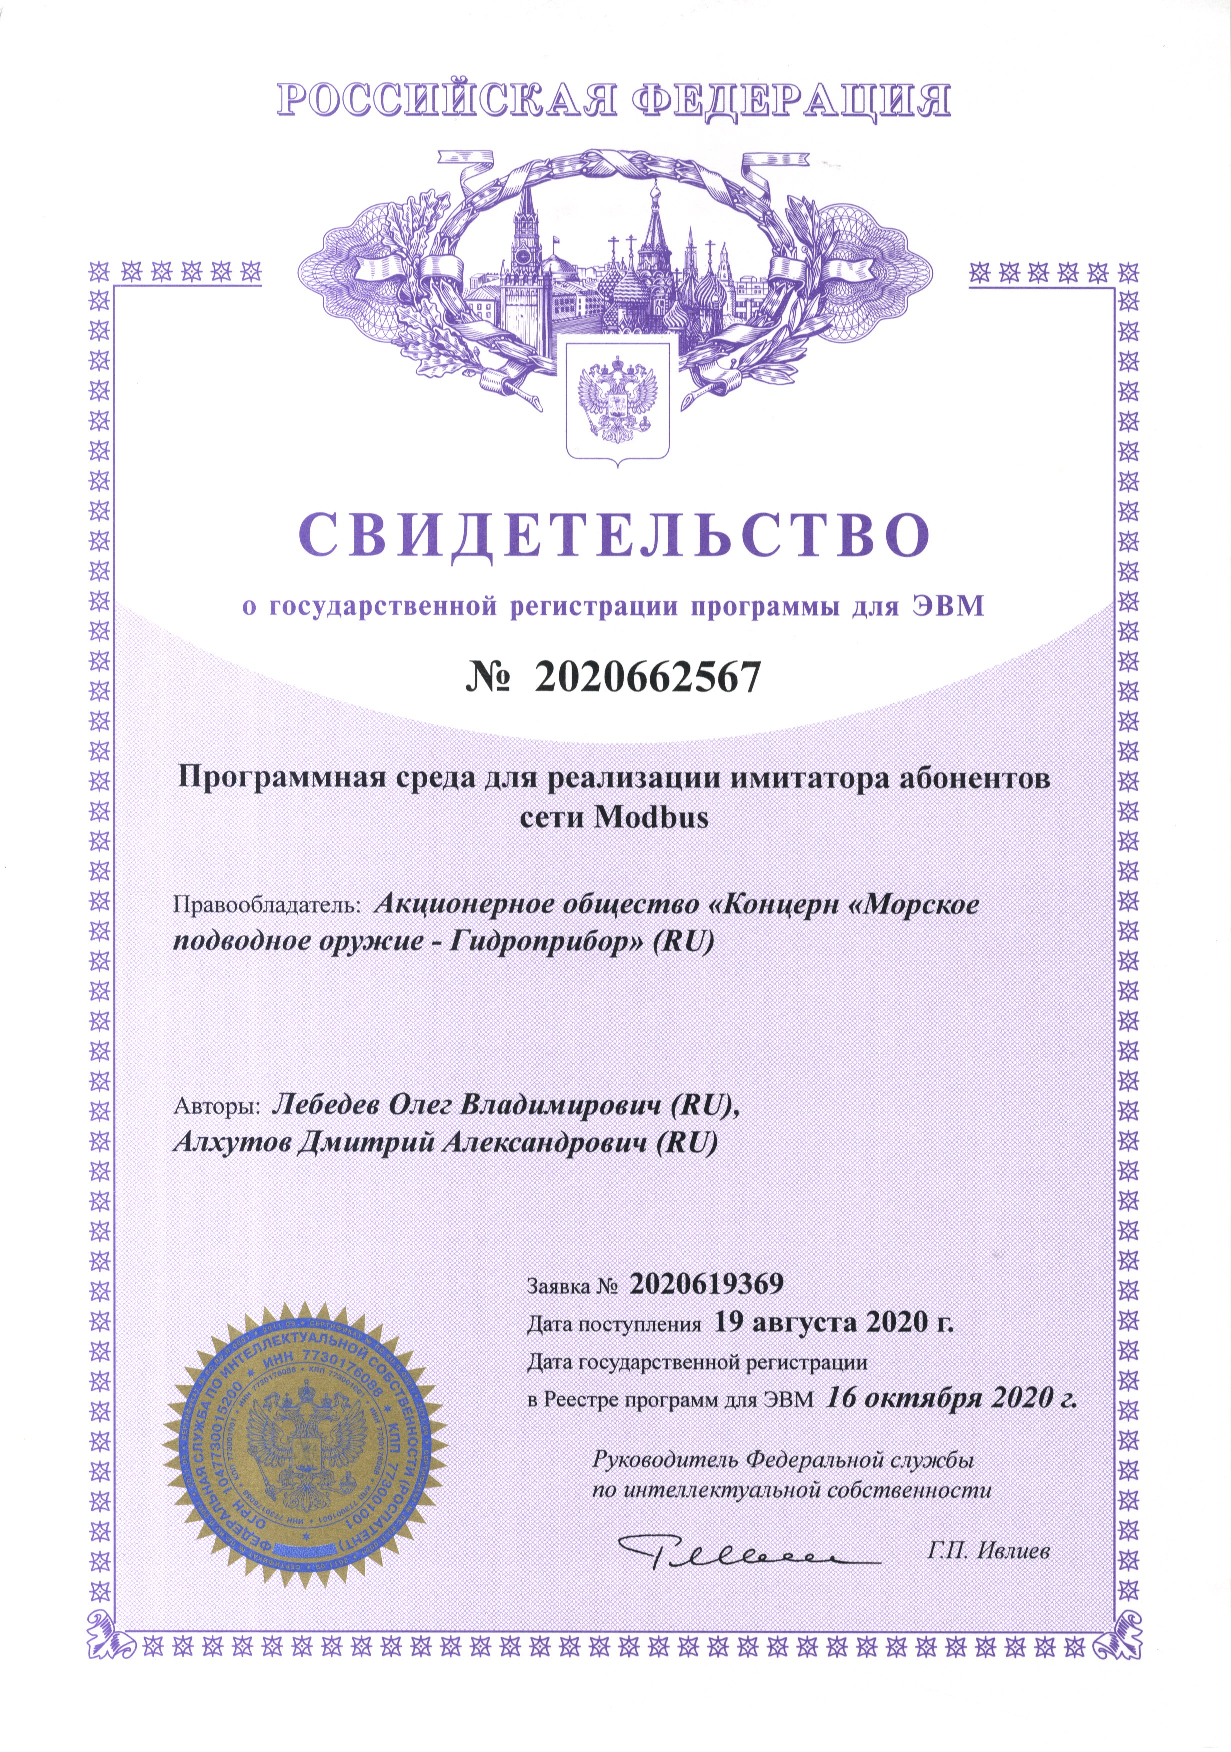
\includegraphics[height=.7\textheight, keepaspectratio]{registration.pdf}
        \caption{Свидетельство о государственной регистрации программы для ЭВМ}\label{app:fig:registration}
    \end{figure}
\end{center}



\chapter{Акт о внедрении}\label{app:sec:implementation}
\begin{center}
    \begin{figure}[hb]
        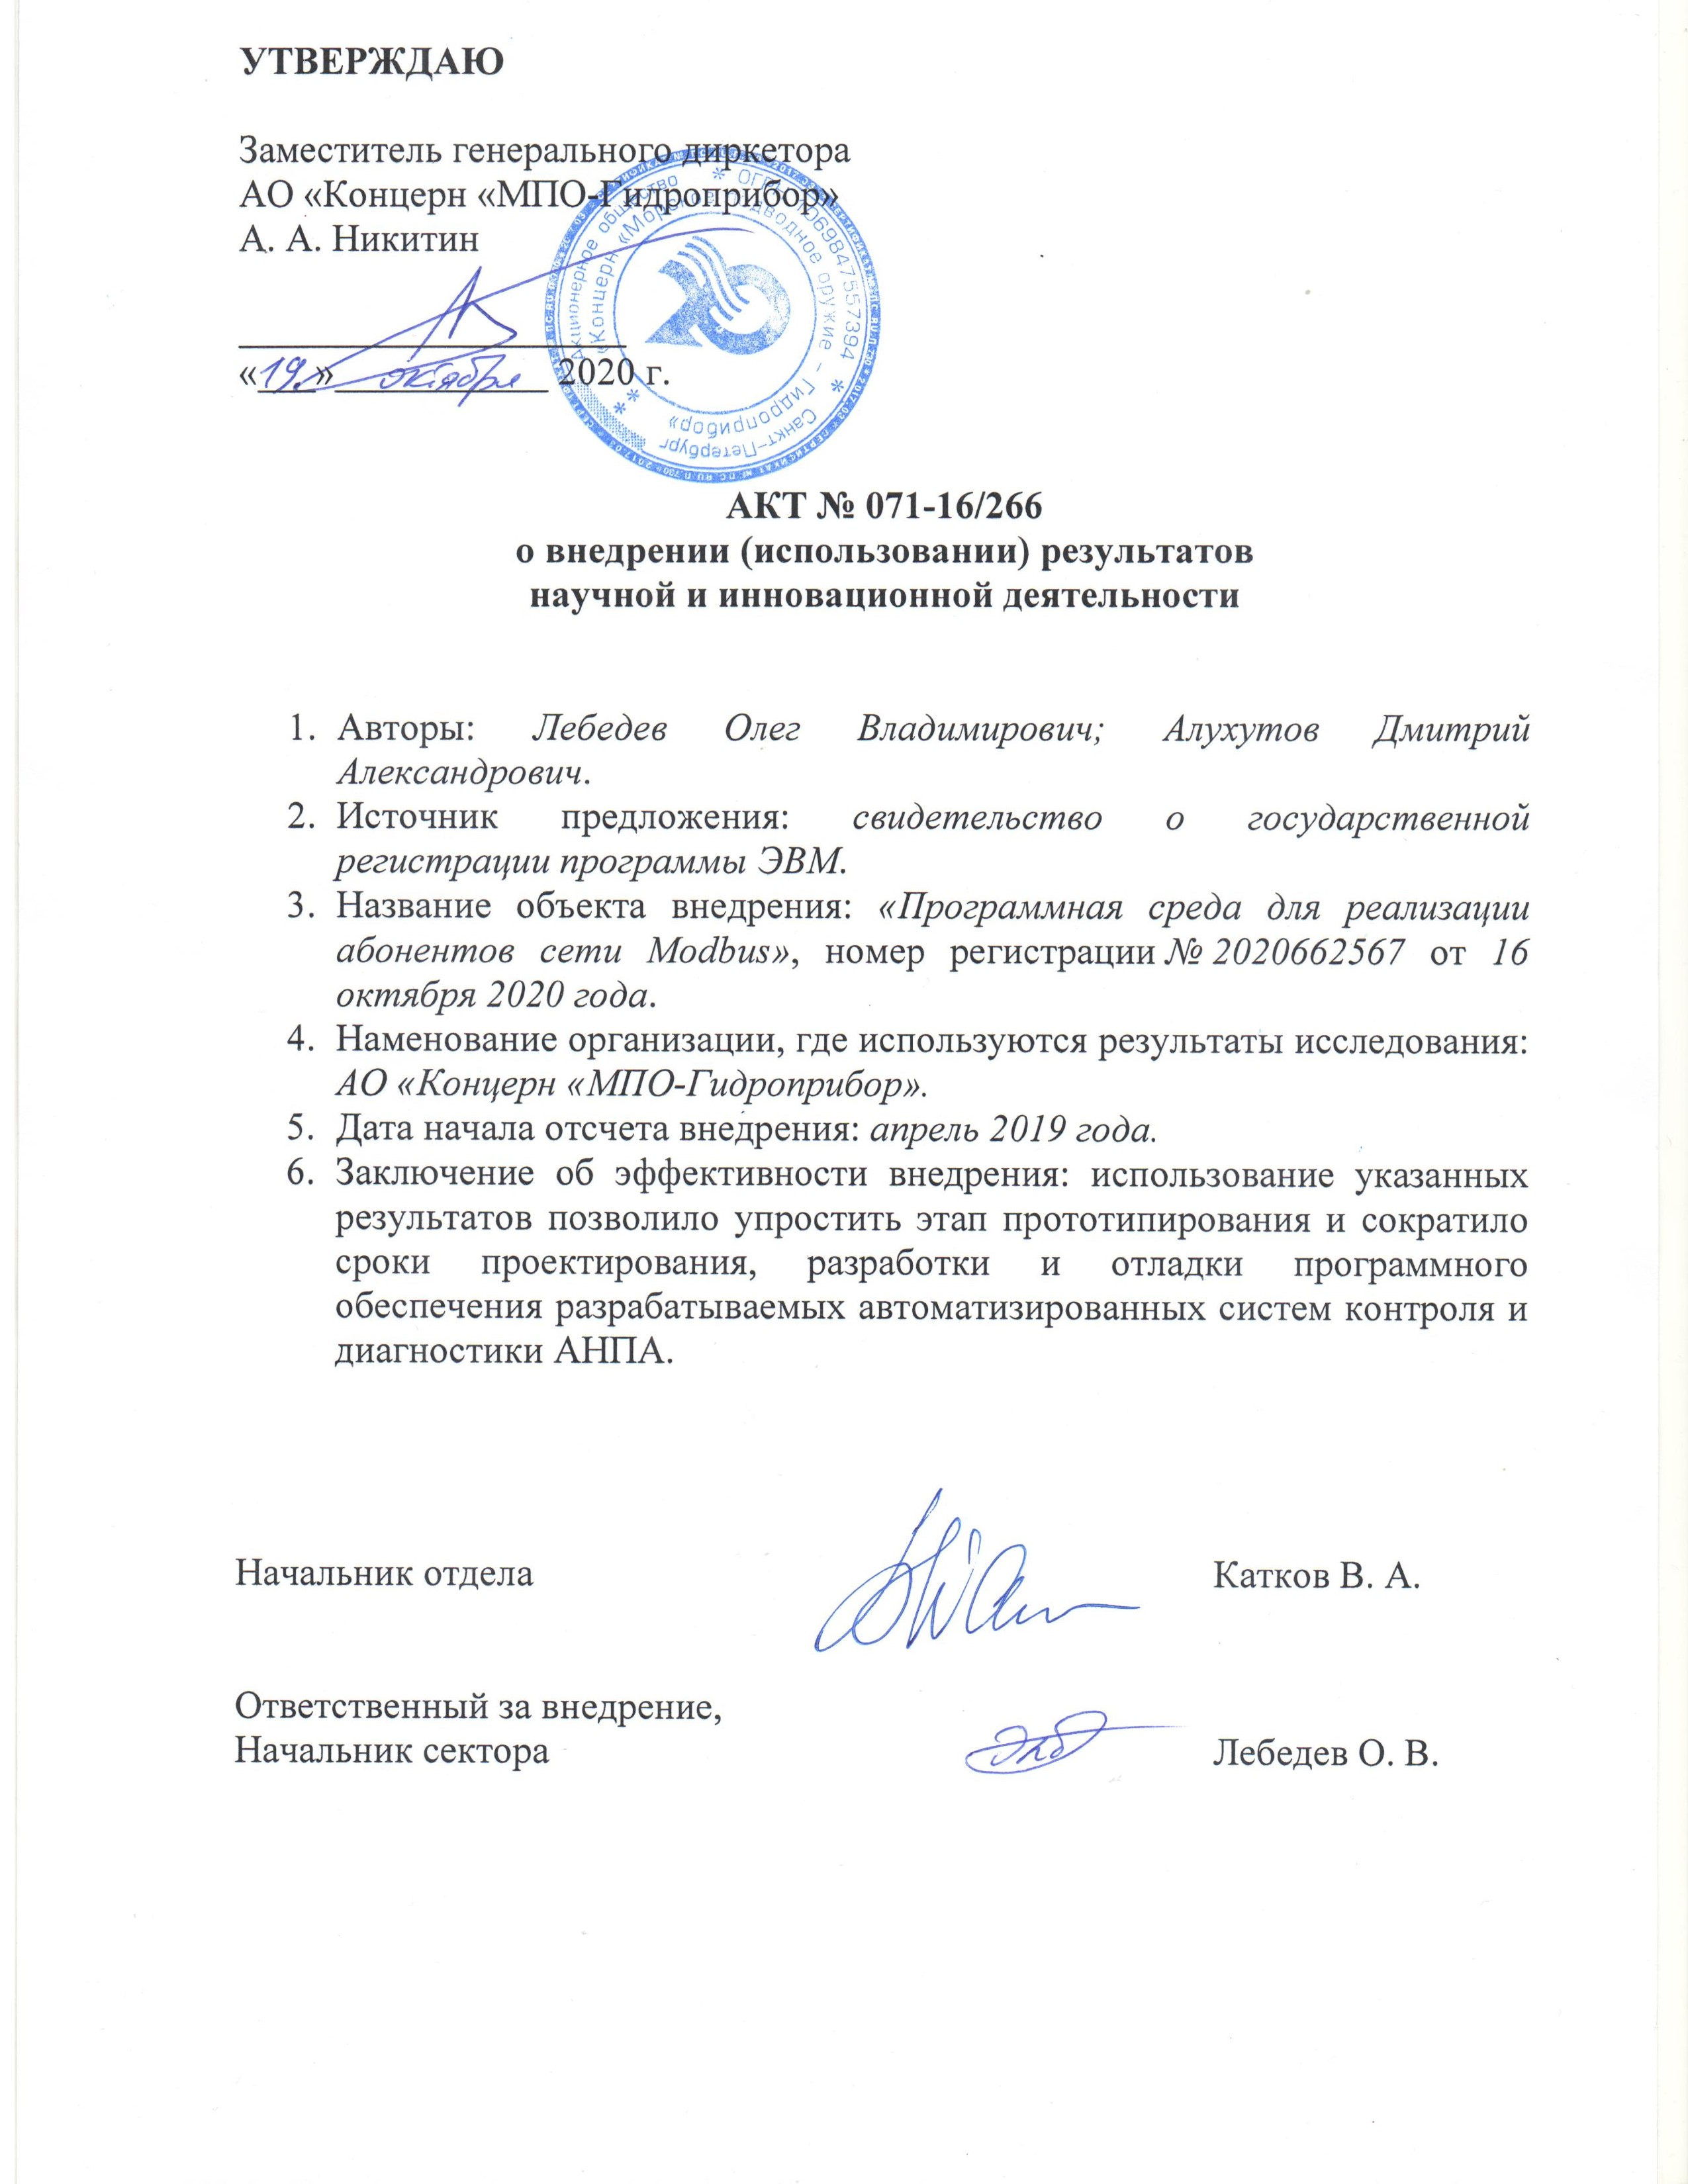
\includegraphics[height=.7\textheight]{implementation}
        \caption{Акт о внедрении на предприятии \leadingOrganizationTitle}\label{app:fig:implementation}
    \end{figure}
\end{center}        % Приложения

\end{document}
